\documentclass{article}
\usepackage[utf8]{inputenc}
%\usepackage{hyperref}
\usepackage[english]{babel}
\usepackage{color}
\usepackage[colorinlistoftodos]{todonotes}
\usepackage{amsmath,amssymb,amsfonts}
\usepackage{amsthm}
\usepackage{enumerate}
\usepackage{enumitem}
\usepackage{array}
\usepackage{multicol}
\usepackage{parskip}
\usepackage{subfiles}
\usepackage[toc,page]{appendix}
\usepackage{graphicx}
\usepackage{subcaption}
\usepackage{tocloft}
\usepackage{titlepic}
\usepackage{wrapfig}
\usepackage{float}
\usepackage{cite}
\usepackage{tabu}
\usepackage{listings}
\usepackage{tikz}
\usepackage[nottoc]{tocbibind}
\usepackage{filecontents}
\usepackage{textcomp}
\usepackage{xcolor}
\usepackage{epstopdf}
\usepackage{caption}
\usepackage{booktabs}
\usepackage{gensymb}
\usepackage[compact]{titlesec}
\usepackage{fancyvrb}
\usepackage{eurosym}
\usepackage{soul}
\usepackage{longtable}
\usepackage[margin=1in]{geometry}
\pagestyle{plain}
\usepackage{hyperref}
\hypersetup{
    colorlinks=true,      % false: boxed links; true: colored links
    linkcolor=black,      % color of internal links (sections, pages, etc.)
    citecolor=black,      % color of citations
    filecolor=black,      % color of file links
    urlcolor=black        % color of external links
}
\definecolor{mygreen}{RGB}{28,172,0} 
\definecolor{mylilas}{RGB}{170,55,241}
\usepackage{lscape}
\usepackage{multirow}
\usepackage{tablefootnote}



\begin{document}
\lstset{language=Matlab,
	basicstyle = \scriptsize,
    breaklines=true,
    morekeywords={matlab2tikz},
    keywordstyle=\color{blue},
    morekeywords=[2]{1}, keywordstyle=[2]{\color{black}},
    identifierstyle=\color{black},
    stringstyle=\color{mylilas},
    commentstyle=\color{mygreen},
    showstringspaces=false,
    numbers=left,
    numberstyle={\small \color{black}},
    numbersep=9pt, 
    emph=[1]{for,end,break},emphstyle=[1]\color{red},   
}


\begin{titlepage}
\begin{center}
{\Large Internship report }\\

\vspace{20mm}

{\bf \textsc{\huge Development of a COMSOL Finite Element Breast Model for Deformation-Based Early Warning Scan Imaging}}\\[8mm]

\bigskip

\begin{figure}[h]
\centering
\begin{minipage}{0.45\linewidth}
    \centering
    
\includegraphics[width=\linewidth]{Figures/Titlepage/tuelogo.png}
\end{minipage}
\hfill
\begin{minipage}{0.45\linewidth}
    \centering
    
\includegraphics[width=\linewidth]{Figures/Titlepage/logo-Catharina-20200701.png}
\end{minipage}
\end{figure}

\begin{figure} [h] 
\includegraphics[width=0.6\linewidth]{Figures/Titlepage/EarlyWarningScan logo.png} \centering \end{figure}

\bigskip



%{\LARGE 30-03-2026  --  12-07-2026}\\[8mm]

% \begin{figure} [h]
% 
\includegraphics[width=0.6\linewidth]{Figures/titlepage.png}
% \centering
% \end{figure}

\vspace{5mm}

{\large By}\\[4mm]
{\large Daan Kuijpers}\\[4mm]
{\large Student number: 1892800}

\vspace{10mm}

{\large Internship at Catharina Hospital Eindhoven}\\[4mm]
{\large 30-03-2026 -- 10-07-2026}

\vspace{10mm}

{\large Catharina Supervisor: Prof. Dr. Ing. Coen Hurkmans}\\[2mm]
{\large TU/e Supervisor: Prof. Dr. Ing. Wouter Huberts}

\vspace{10mm}



%%Datum van inleveren laatste bewerking onderaan pagina
\large Eindhoven, \today \\
\end{center}
\end{titlepage}


\newpage
\begingroup
\small
\setlength{\parskip}{0pt}
\setlength{\baselineskip}{11pt}
\tableofcontents
\endgroup

\newpage
\section{Abstract}

This internship project developed a reproducible COMSOL finite-element workflow for modelling dynamic breast deformation in the context of the Early Warning Scan. The work focused on improving a parametrised breast model by adding a curved posterior support, a more realistic fibroglandular tissue distribution, volumetric skin representation, material-sensitivity routes, simplified Cooper-like support and analytic tumor-overlay placement.

The workflow generated traceable COMSOL model variants and compact post-processing outputs for comparing selected modelling choices. Material and skin-parameter changes produced the strongest displacement differences in the available result sets, while the simplified Cooper-like support variants produced only small global displacement changes. The tumor-overlay route was implemented and visualised at build level for different tumor sizes and locations, but the current results should not be interpreted as evidence of tumor detectability.

The main limitation was computational capacity, because time-dependent simulations and post-processing were performed on local hardware. The developed workflow therefore provides a model-development platform for future EWS-oriented deformation studies, but further work should use stronger computational resources, larger matched simulation sets and experimental or EWS-like validation data.
\newpage
\section{Introduction}

Breast cancer is the most commonly diagnosed cancer among women worldwide, with more than 2.3 million new cases reported annually \cite{WHO2025}. Early detection is essential for improving treatment options and patient outcome. X-ray mammography is currently the standard method for population-based breast cancer screening, but it also has relevant limitations. In particular, mammographic sensitivity is reduced in women with dense breast tissue, where the contrast between lesions and surrounding fibroglandular tissue can be limited \cite{VonEuler-Chelpin2019, Bakker2019}. In addition, mammography uses ionizing radiation and requires breast compression, which motivates continued research into complementary, non-invasive and radiation-free screening approaches.

\subsection{Background}

One possible direction for radiation-free breast cancer detection is to use the mechanical contrast between healthy and pathological tissue. Malignant breast tumours are generally stiffer than surrounding adipose and fibroglandular tissue, although reported stiffness values vary with measurement technique, loading condition and tissue type \cite{Samani2007, Ramiao2016, Goodbrake2022}. This mechanical contrast forms the basis for elastography-based imaging techniques, in which tissue deformation is used to infer differences in internal mechanical properties \cite{Patel2022, Patel2021, Jamshidi2024}.

This project was performed in collaboration with Early Warning Scan (EWS), which is developing a non-invasive screening concept based on optical and biomechanical measurements of breast deformation \cite{EarlyWarningScanWebsite}. The underlying principle is related to Digital Image Elasto-Tomography (DIET), where the breast is mechanically excited and the resulting surface motion is captured using optical measurements. Differences in internal stiffness may then affect the measured surface displacement field and dynamic response \cite{Peters2004, VanHouten2011, Fitzjohn2022}. Previous phantom and modelling studies have shown that finite element (FE) models can support the development of DIET-like systems by generating controlled deformation data and by testing the effect of stiff inclusions under known conditions \cite{Kashif2013, Ismail2018}.

Finite element method (FEM) modelling is widely used to study breast biomechanics because it allows geometry, material properties, boundary conditions and loading conditions to be controlled independently. Early breast FEM studies already demonstrated the usefulness of three-dimensional biomechanical models for simulating breast deformation and image-related applications \cite{Samani2001, Hsu2011}. More recent work has moved toward patient-specific and multi-component models that include separate anatomical regions such as adipose tissue, fibroglandular tissue, skin, muscle and support structures, each with distinct mechanical properties \cite{Samani2001, Hsu2011, Chen2024, Mazier2024}. Such models can be used to study breast motion, compression, gravity-induced deformation, image registration and the effect of internal tissue composition on the external deformation response.

However, breast modelling remains challenging. Breast tissue is heterogeneous, nonlinear and individual-specific, and its mechanical properties vary substantially between studies, measurement protocols and anatomical regions \cite{Ramiao2016, Goodbrake2022, Galbreath2025, Teixeira2023}. Anatomical features such as the posterior chestwall interface, fibroglandular distribution, skin layer and Cooper-ligament support can all influence the simulated deformation response. At the same time, adding anatomical detail increases model complexity, solver cost and the risk of poorly controlled comparisons. For an EWS-oriented modelling workflow, it is therefore important not only to make the model more realistic, but also to keep the development process reproducible and interpretable.

\subsection{Objectives}

The aim of this internship project was to develop a reproducible COMSOL-based FEM pipeline for a parametrised breast model and to use this pipeline to investigate how selected anatomical and mechanical modelling choices influence the simulated deformation response. The project started from the objective of improving the realism of an existing breast model, with an initial emphasis on geometry, posterior chestwall support and internal tissue representation. The focus was not to create a final patient-specific diagnostic model, but to establish a controlled model-development workflow in which model variants can be generated, solved and compared systematically.

The central research question of this project was:

\begin{quote}
How do controlled changes in chestwall geometry, glandular tissue distribution, outer breast shape, support representation, material settings and tumor inclusion affect the simulated displacement and stress response of a heterogeneous finite element breast model?
\end{quote}

To address this question, the model was developed in a staged manner. The first stages focused on establishing a stable dynamic baseline and improving the anatomical description of the model through the posterior chestwall geometry and glandular tissue distribution. Subsequent stages introduced matched controls for outer-shape asymmetry and Cooper-ligament support, followed by material and skin-layer sensitivity cases and an initial tumor screening route. This staged structure was chosen to make the effect of individual modelling assumptions easier to interpret.

COMSOL Multiphysics was used as the intended modelling environment for this project, but an important part of the work was to determine whether a sufficiently automated and reproducible COMSOL workflow could be built for this type of parametrised breast model \cite{COMSOLMultiphysicsWebsite}. The resulting pipeline supports systematic comparison between model variants while keeping the model definitions and evaluation outputs traceable. The final outcome of the project is therefore a reproducible COMSOL FEM model-development pipeline for EWS-oriented breast deformation studies, together with a critical assessment of which model components are suitable for quantitative interpretation and which should still be considered exploratory model-development results.


\newpage
\section{Materials and Methods}


%%%%%%%%%%%%%%%%%%%%%%%%%%%%%
% SECTION 3.1 BELOW
%%%%%%%%%%%%%%%%%%%%%%%%%%%%%


\subsection{Model-development workflow}

\subsubsection{Starting point and relation to previous EWS FEM work}

This project was developed in the context of previous internal EWS finite element modelling work. Earlier EWS models provided a useful methodological starting point for breast geometry parameterisation, soft-tissue material assumptions, dynamic loading and displacement-based evaluation \cite{EngelsEWSReport, StormEWSReport}. These previous projects were used as engineering reference material and as a comparison point for modelling choices. They were not used as validation datasets for the current COMSOL model.

The present project develops a separate COMSOL-based modelling route. The motivation for this route was to improve control over constructive geometry, region definitions, model variants and post-processing while keeping the workflow reproducible. This was especially relevant because the project aimed to investigate the influence of individual anatomical and mechanical components, including chestwall shape, fibroglandular tissue distribution, skin representation, Cooper-ligament support approximation and tumor inclusion. Additional context on the previous EWS FEM work is provided in Appendix~\ref{sec:appendix_previous_ews_fem_work}, while the current repository structure is summarised in Appendix~\ref{sec:appendix_current_repository}.

\subsubsection{COMSOL-based workflow}

The finite element model was implemented in COMSOL Multiphysics and controlled using a Python-based source-case workflow \cite{COMSOLMultiphysicsWebsite}. Each model variant was defined by a case configuration file containing the main geometry, material, loading and evaluation settings. These settings were used to generate a consistent COMSOL model definition, including the required geometry operations, material assignments, selections, study settings and post-processing outputs. An overview of the workflow is shown in Figure~\ref{fig:comsol_pipeline_overview}.

\begin{figure}[H]
\centering
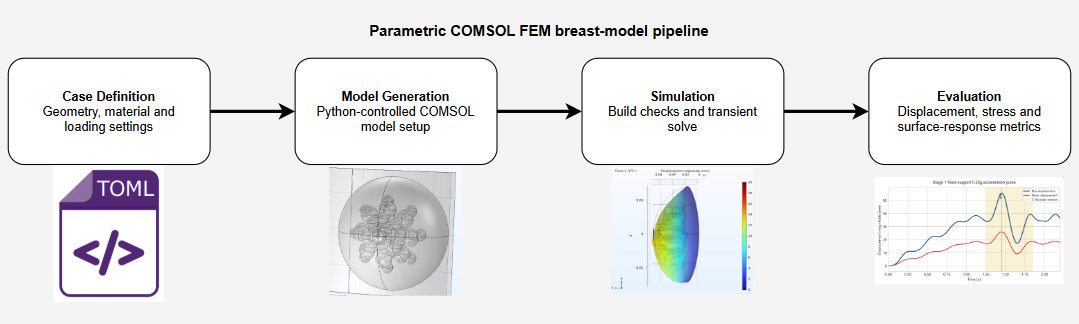
\includegraphics[width=0.95\linewidth]{Figures/M&M/model_overviews/Report_pipeline_overview.png}
\caption{Overview of the COMSOL-based model-development workflow. Case definitions specify the main geometry, material and loading settings. These settings are used by the Python-controlled workflow to generate the COMSOL model, perform build and solve steps, and export compact evaluation outputs for comparison.}
\label{fig:comsol_pipeline_overview}
\end{figure}

The purpose of this workflow was to make model changes traceable. Instead of manually modifying a COMSOL model for each comparison, the relevant modelling assumptions were stored in version-controlled case definitions. This allowed related model variants to be generated from a consistent structure and made it easier to identify which modelling change was responsible for a difference in the simulated displacement or stress response. The project repository contains the implementation of the Python workflow, the active TOML case definitions and the compact evaluation outputs used for the comparisons \cite{KuijpersEWSComsolGitHub}. These case definitions were used to keep the modelling assumptions for each variant traceable without relying on manual edits to a single COMSOL model file.

\subsubsection{Model-development strategy}

The model was developed by adding and testing one modelling component at a time. The development was organised around six main modelling themes: dynamic excitation, posterior chestwall geometry, internal fibroglandular tissue distribution, outer-shape variation, mechanical support representation and tumor sensitivity. This structure was used to reduce the risk of interpreting multiple model changes at once.

The first part of the workflow focused on establishing a stable dynamic input and a controlled anatomical reference geometry. The posterior support was then refined using a curved chestwall representation, followed by a more detailed fibroglandular tissue distribution. After this anatomical route was established, additional model variants were used to investigate outer-shape asymmetry, Cooper-ligament support approximations, and skin and material sensitivity. Tumor sensitivity was treated as a separate final extension of the workflow. In this extension, spherical tumor-overlay definitions were prepared for different sizes and locations to test whether local stiffness inclusions could be added consistently to the existing COMSOL model. The overall model-development route is summarised in Figure~\ref{fig:model_development_route}.

\begin{figure}[H]
\centering
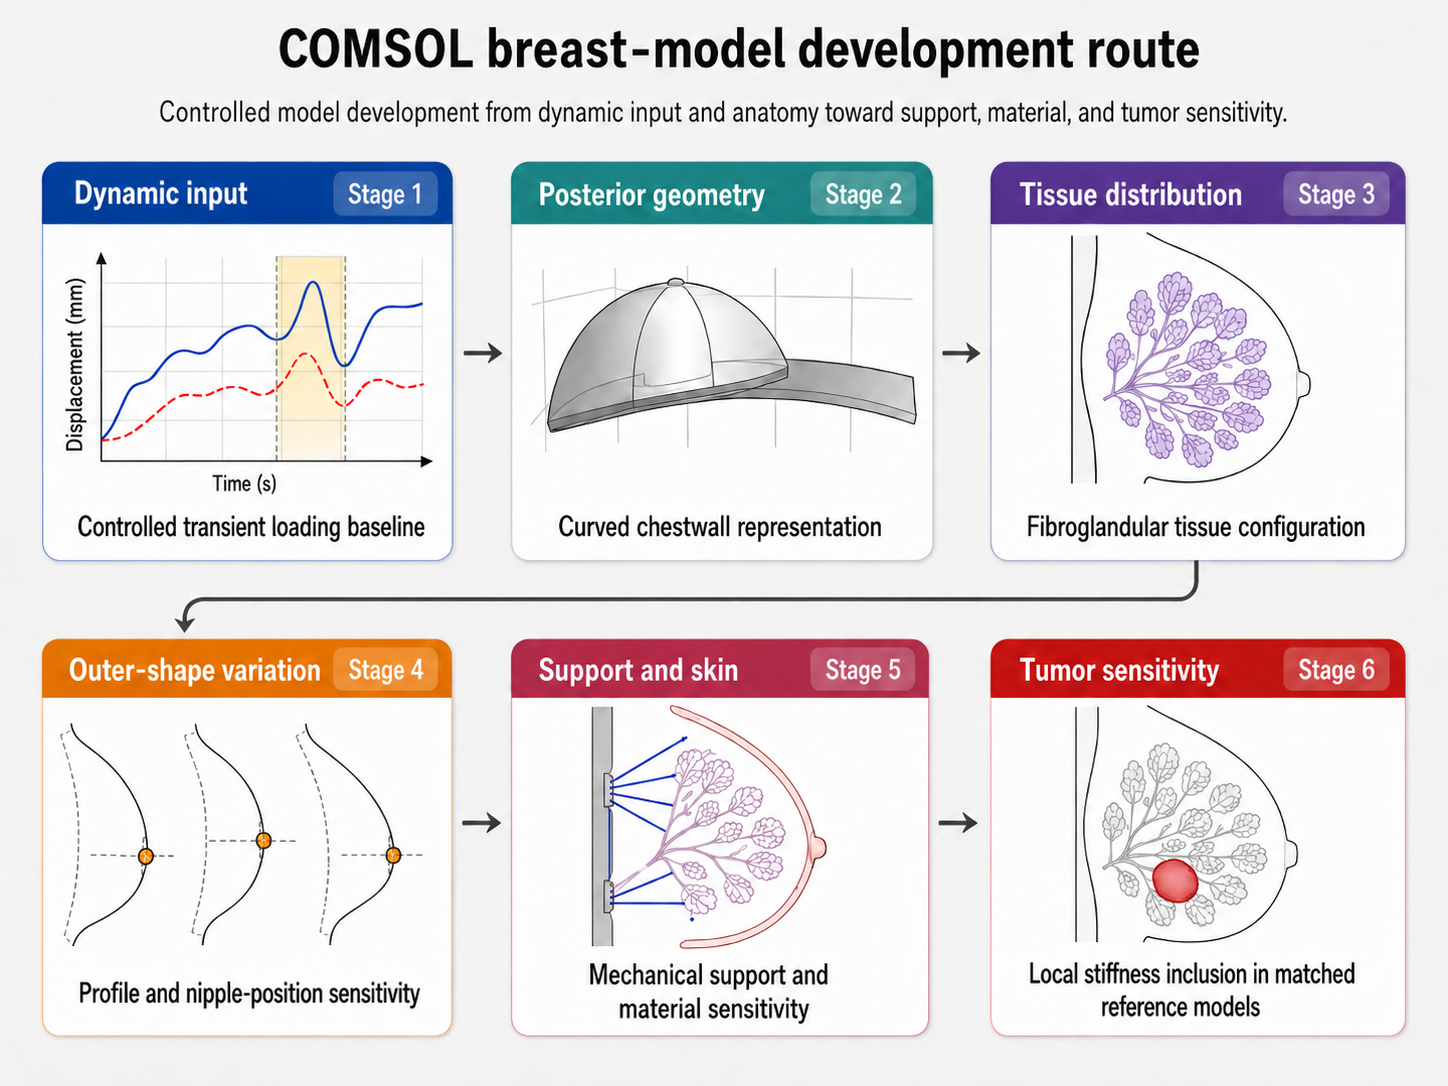
\includegraphics[width=0.95\linewidth]{Figures/M&M/model_overviews/report_staged_model_overview.png}
\caption{Schematic overview of the COMSOL breast-model development route used in this project. The workflow progresses from dynamic input and anatomical model definition toward outer-shape variation, support and skin sensitivity, and tumor sensitivity, allowing individual modelling components to be investigated in a controlled manner.}
\label{fig:model_development_route}
\end{figure}

Not all model variants had the same interpretation status. Some cases were used as controlled reference models for quantitative comparison, whereas others were used as exploratory checks for numerical stability, geometry construction or sensitivity to modelling assumptions. This distinction is important because the aim of the project was not to validate a final patient-specific diagnostic model, but to construct a reproducible COMSOL FEM workflow and to identify which modelling components have a measurable influence on the simulated breast deformation response.


%%%%%%%%%%%%%%%%%%%%%%%%%%%%%
% SECTION 3.2 BELOW
%%%%%%%%%%%%%%%%%%%%%%%%%%%%%


\subsection{Anatomical model definition}
\label{sec:anatomical_model_definition}

The anatomical model was defined as a parametrised breast representation rather than as a reconstruction of one individual patient. This choice reflects the aim of the EWS modelling workflow to generate controlled breast-model variants that can be used to study how anatomy, tissue distribution, material assumptions and tumor properties affect the simulated surface deformation response. In the longer term, such a parametrised modelling route could support the generation of synthetic deformation data for algorithm development and AI training, provided that the simulated responses are sufficiently well understood and validated. Patient-specific breast geometries remain important for clinical modelling applications \cite{Samani2001,Hsu2011,Mazier2024}, but the present work focuses on building a reproducible model-development platform that can later be extended toward broader anatomical variation and more patient-specific inputs.

In this section, the anatomical definition is limited to the geometric and tissue-layout components of the model. This includes the parametrised breast envelope, posterior chestwall representation, fibroglandular tissue distribution, and controlled outer-shape and nipple-position variations. Anatomically motivated components that were implemented mainly through material or support definitions, such as the skin layer, Cooper-ligament support approximation and tumor inclusion, are described in Section~\ref{sec:mechanical_model_definition}.

\subsubsection{Parametrised breast geometry and reference volume}
\label{sec:parametrised_breast_geometry}

The overall breast shape was generated from the TOML case-definition parameters used by the COMSOL pipeline. For the selected anatomical route, the model used a characteristic radius of 70~mm, an elliptic outer profile, an anterior projection scale of 1.08 and a superior-pole scale of 0.98. The radius sets the global model scale, while the profile and scaling factors adjust the anterior projection and upper-breast shape. These parameters were selected as representative model-construction settings for the reference geometry.

The reference volume was chosen by comparing the generated COMSOL geometry with literature values for breast-volume measurement and with an internal Catharina Hospital dataset of 100 manually delineated breast volumes \cite{Stahl2023,Yoo2013,Nie2010SkinRemoval,Choppin2016}. The details of this comparison are provided in Appendix~\ref{sec:appendix_breast_volume_reference}. Because breast-volume estimates depend on measurement method, patient position and boundary definition, the selected volume was not treated as a single population average, but as a defensible reference size for controlled model development.

After the COMSOL geometry operations, including posterior support construction and volume-preserving compensation, the selected anatomical route produced a breast volume of $\sim$585~mL. This value is within the lower-mid range of the internal dataset and is consistent with the literature-based volume context. It was therefore used as a controlled reference volume for the main matched comparisons. Keeping this volume fixed prevented later changes in tissue distribution, asymmetry, support representation or tumor inclusion from being combined with a change in overall breast size.

\subsubsection{Posterior chestwall representation}
\label{sec:posterior_chestwall_representation}

The posterior boundary of the breast was represented by a simplified chestwall support geometry. This support was not intended as a full anatomical reconstruction of the thoracic wall or pectoral region, but as a controlled posterior interface that better reflects the curved support on which the breast rests than the flat chestwall used in earlier internal EWS modelling work. Curved posterior support is also consistent with breast FEM literature, where the breast is commonly modelled relative to the thoracic wall, pectoral region or posterior support boundary \cite{Hsu2011,Mazier2024}.

In the selected reference route, the posterior support was implemented as a transverse curved support geometry with volume-preserving compensation, as shown in Figure~\ref{fig:chestwall_reference_geometry}. In the COMSOL case definition, this route used the support mode \texttt{transverse\_vp}, a transverse curve depth of 21~mm and a chestwall-curve centre offset of +55~mm in the COMSOL $x$-direction. The posterior support was generated using a \texttt{cylinder\_band} geometry, such that the chestwall shape could be adjusted through the curvature depth and offset parameters. A positive offset represents the selected left-breast orientation used in this report route, while the same construction can be mirrored using a negative offset for a right-breast orientation.

\begin{figure}[H]
\centering
\begin{subfigure}{0.48\linewidth}
\centering
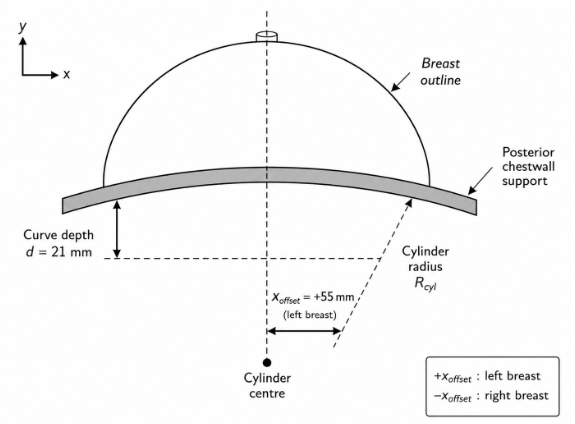
\includegraphics[width=\linewidth]{Figures/M&M/Schematic_chestwall_parameters.png}
\caption{Schematic top view}
\end{subfigure}
\hfill
\begin{subfigure}{0.48\linewidth}
\centering
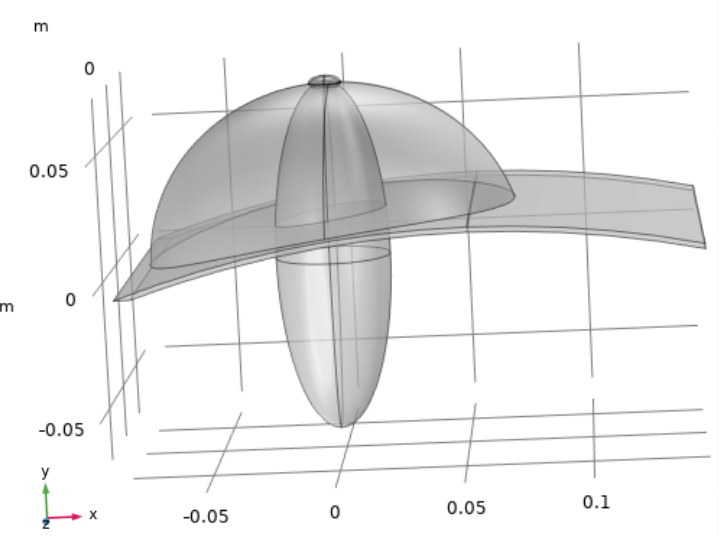
\includegraphics[width=\linewidth]{Figures/M&M/Superior_chestwallcurve.png}
\caption{COMSOL-rendered superior view}
\end{subfigure}
\caption{Posterior chestwall representation used in the selected reference route. The schematic view illustrates the transverse curved support geometry, including the curvature depth and the $x$-offset of the cylinder centre. The COMSOL-rendered view shows the corresponding curved posterior support geometry for the selected $+55~\mathrm{mm}$ chestwall-offset configuration.}
\label{fig:chestwall_reference_geometry}
\end{figure}

Superior--inferior curvature can also be combined with the transverse support geometry in the pipeline. However, this additional curvature was not retained in the selected reference baseline because the transverse curvature represented the dominant anatomical refinement compared with the earlier flat chestwall, while exploratory COMSOL checks showed only a limited additional effect from the superior--inferior component. Excluding this extra curvature also kept the reference geometry simpler and more stable for the matched comparisons. To preserve geometric consistency across parameter choices, the nipple-related helper geometry and anterior glandular alignment were updated automatically relative to the selected chestwall shape using projected-normal alignment.


\subsubsection{Fibroglandular tissue distribution}
\label{sec:fibroglandular_tissue_distribution}

The fibroglandular tissue representation was refined from a simple internal region toward a more structured lobule-based distribution. This step was included to make the internal tissue layout more anatomically realistic, because breast tissue is heterogeneous and internal tissue composition can influence the simulated deformation response \cite{Chen2024,Mazier2024}.

The selected reference route was guided mainly by the multi-component breast-model approach described by Chen et al. \cite{Chen2024}. In the COMSOL implementation, the fibroglandular region was generated using the \texttt{chen\_2024\_template\_lobes} mode. The reference configuration used 12 lobules, divided into 4 inner and 8 outer lobules, with duct-like components directed toward the nipple, a subareolar core and a subareolar bridge. A lateral view of the reference configuration is shown in Figure~\ref{fig:fibroglandular_reference_lateral}.

Three spread variants were retained: compact, reference and wide. These variants changed the spatial spread of the lobules while keeping the selected Stage~2 chestwall geometry and the same general model setup. The reference spread was used as the main anatomical route for later comparisons, while the compact and wide variants were used to check the geometric effect of the assumed fibroglandular spread. The compact and wide variants are shown in Figure~\ref{fig:fibroglandular_spread_variants}.

The current reference model had a total breast volume of $\sim$585~mL and used a glandular fraction of $\sim$24.3\%, corresponding to a glandular volume of $\sim$142.2~mL. This value was considered acceptable for the reference route after comparison with literature on volumetric breast density and fibroglandular tissue quantification \cite{Sartor2016,Nie2010,Lu2012}. Because volumetric fibroglandular fraction is not directly equivalent to projected mammographic density or to the Breast Imaging Reporting and Data System (BI-RADS) breast-composition categories, the literature context is summarised separately in Appendix~\ref{sec:appendix_glandular_fraction_reference} \cite{ACRBIRADS}. The resulting reference and spread-variation layouts are shown in Figure~\ref{fig:fibroglandular_distribution_variants}.

\begin{figure}[H]
\centering
\begin{subfigure}{0.32\linewidth}
\centering
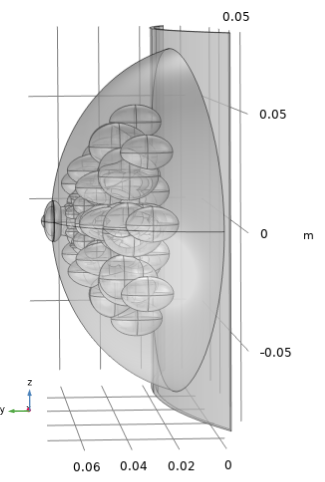
\includegraphics[width=\linewidth,height=0.24\textheight,keepaspectratio]{Figures/M&M/leftantroir_view_gland.png}
\caption{Reference lateral view}
\label{fig:fibroglandular_reference_lateral}
\end{subfigure}
\hfill
\begin{subfigure}{0.64\linewidth}
\centering
\begin{minipage}{0.48\linewidth}
\centering
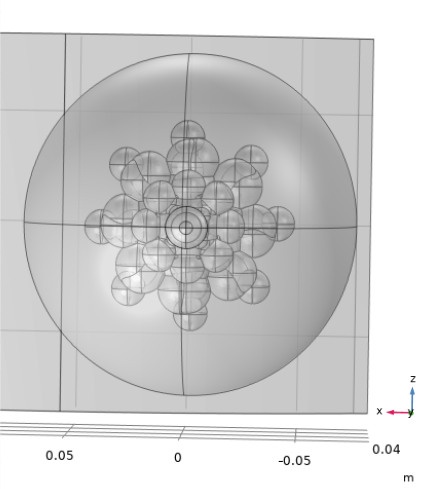
\includegraphics[width=\linewidth]{Figures/M&M/compact_spread.png}
\end{minipage}
\hfill
\begin{minipage}{0.48\linewidth}
\centering
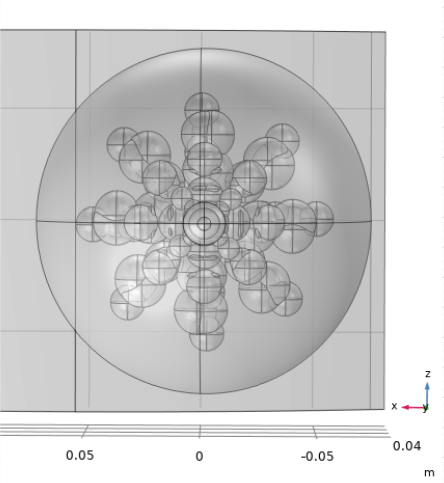
\includegraphics[width=\linewidth]{Figures/M&M/wide_spread.png}
\end{minipage}
\caption{Compact (left) and wide (right) anterior views}
\label{fig:fibroglandular_spread_variants}
\end{subfigure}

\caption{COMSOL-rendered fibroglandular tissue configurations used in the Stage~3 anatomical route. The reference lateral view shows the chestwall-aware lobule and duct structure inside the selected $+55~\mathrm{mm}$ chestwall-offset geometry. The compact and wide anterior views illustrate the spread variants used to evaluate the effect of fibroglandular spatial distribution.}
\label{fig:fibroglandular_distribution_variants}
\end{figure}

\subsubsection{Outer-shape and nipple-position variations}
\label{outer_shape_nipple_variations}

Outer-shape and nipple-position variations were included because breast size, shape and left--right symmetry vary substantially between individuals \cite{Stahl2023,Mazier2024}. For an EWS-oriented model, this is relevant because surface shape and nipple position influence both the visible breast surface and the interpretation of local displacement or landmark motion.

Stage~4 was therefore used to test controlled geometry variations on top of the selected Stage~2 chestwall geometry and Stage~3 fibroglandular reference. In the COMSOL case definitions, the outer breast shape can be scaled in width and height, while the nipple position can be shifted over the breast surface in the $x$- and $z$-directions. Examples of these geometry variations are shown in Figure~\ref{outer_shape_nipple_variation_examples}.

For nipple-position variations, the associated lobules, ducts, subareolar core and bridge were updated relative to the final nipple axis, so that the internal fibroglandular layout remained coupled to the shifted nipple position. These cases were used as controlled geometry-sensitivity previews and should not be interpreted as patient-specific asymmetry reconstructions.


\begin{figure}[H]
\centering
\begin{subfigure}{0.32\linewidth}
\centering
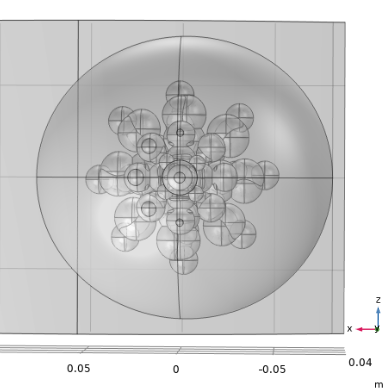
\includegraphics[width=\linewidth]{Figures/M&M/scaling.png}
\caption{Profile scaling (widening)}
\label{stage4_profile_scaling_panel}
\end{subfigure}
\hfill
\begin{subfigure}{0.32\linewidth}
\centering
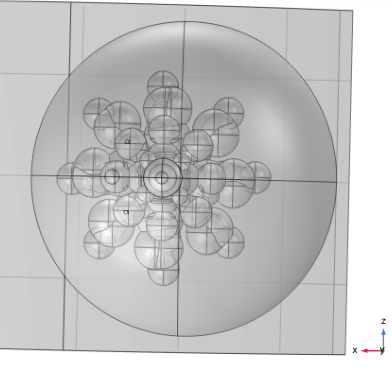
\includegraphics[width=\linewidth]{Figures/M&M/lateral_nipple.png}
\caption{Lateral nipple shift}
\label{stage4_lateral_nipple_shift_panel}
\end{subfigure}
\hfill
\begin{subfigure}{0.32\linewidth}
\centering
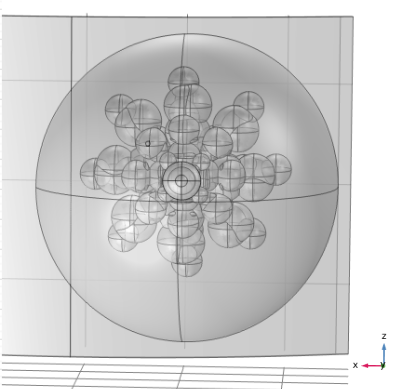
\includegraphics[width=\linewidth]{Figures/M&M/superior_nipple.png}
\caption{Superior nipple shift}
\label{stage4_superior_nipple_shift_panel}
\end{subfigure}

\caption{COMSOL-rendered examples of the outer-shape and nipple-position variation cases used in Stage~4. The cases test controlled changes in breast profile and nipple position while preserving the selected Stage~2 chestwall route and Stage~3 fibroglandular reference.}
\label{outer_shape_nipple_variation_examples}
\end{figure}




%%%%%%%%%%%%%%%%%%%%%%%%%%%%%
% SECTION 3.3 BELOW
%%%%%%%%%%%%%%%%%%%%%%%%%%%%%


\subsection{Mechanical model definition}
\label{sec:mechanical_model_definition}

The mechanical model defines how the anatomical regions described in Section~\ref{sec:anatomical_model_definition} were assigned material behaviour and mechanical support assumptions in COMSOL. The workflow was organised into separate material and support routes, so that the influence of individual modelling choices, including tissue stiffness, skin representation, Cooper-ligament support and tumor inclusion, could be evaluated independently from the anatomical geometry. This separation allowed the mechanical contribution of each model component to be tested without redefining the underlying segmented breast shape.

\subsubsection{Constitutive material model}
\label{constitutive_material_model}

Breast tissue was modelled as a soft, nearly incompressible material. This is consistent with common breast FEM practice, although reported mechanical properties vary substantially between studies because of differences in measurement protocol, preload, strain level, tissue type and constitutive model \cite{Samani2007,Ramiao2016,Goodbrake2022,Teixeira2023}. In the COMSOL source-case definition, adipose, fibroglandular, skin and tumor materials were parameterised using density, bulk modulus $K$ and two Mooney--Rivlin-type coefficients, $C_{10}$ and $C_{01}$. Related Mooney--Rivlin-type soft-tissue material descriptions were also used in previous internal EWS/FEBio modelling work, which served as historical reference material for the current COMSOL route \cite{EngelsEWSReport,StormEWSReport}.

The source material parameterisation can be written in terms of a deviatoric Mooney--Rivlin strain-energy density with an additional volumetric contribution \cite{Mooney1940,Rivlin1948},

\begin{equation}
W
=
C_{10}\left(\bar{I}_{1}-3\right)
+
C_{01}\left(\bar{I}_{2}-3\right)
+
W_{\mathrm{vol}}\left(J;K\right).
\label{mooney_rivlin_strain_energy_density}
\end{equation}

Here, $\bar{I}_{1}$ and $\bar{I}_{2}$ are the modified invariants, $J$ is the volume ratio and the volumetric part is controlled by the bulk modulus $K$. Equation~\ref{mooney_rivlin_strain_energy_density} describes the source material parameterisation used in the workflow. It should not be interpreted as a full derivation of the exact volumetric penalty formulation used internally by COMSOL.

For stiffness-scale interpretation, and for the effective small-strain material route used where the COMSOL implementation requires linear-elastic quantities, the Mooney--Rivlin source parameters were mapped to equivalent small-strain elastic constants using:

\begin{equation}
G_{0}
=
2\left(C_{10}+C_{01}\right),
\label{small_strain_shear_modulus_from_mooney_rivlin}
\end{equation}

\begin{equation}
E
=
\frac{9KG_{0}}{3K+G_{0}},
\label{small_strain_youngs_modulus_from_bulk_and_shear}
\end{equation}

and

\begin{equation}
\nu
=
\frac{3K-2G_{0}}{2\left(3K+G_{0}\right)}.
\label{small_strain_poisson_ratio_from_bulk_and_shear}
\end{equation}

The coefficients $C_{10}$ and $C_{01}$ determine how strongly the Mooney--Rivlin material resists shape change at small deformation. Their sum gives the small-strain shear modulus $G_{0}$. This shear modulus was then combined with the bulk modulus $K$, which controls resistance to volume change, to obtain an equivalent Young's modulus $E$ and Poisson's ratio $\nu$ for small-strain interpretation. Because soft breast tissue was treated as nearly incompressible, $K$ was chosen much larger than $G_{0}$, resulting in $\nu$ close to $0.5$.

For nearly incompressible behaviour, where $K$ is much larger than $G_{0}$, this reduces approximately to

\begin{equation}
E
\approx
3G_{0}
=
6\left(C_{10}+C_{01}\right).
\label{nearly_incompressible_stiffness_scale}
\end{equation}

The resulting stiffness value $E$ was therefore reported as a small-strain equivalent stiffness, allowing the material sets to be compared more directly with each other and with literature values commonly reported in terms of Young's modulus. It does not replace the original Mooney--Rivlin source-parameter definition. The posterior chestwall support was represented separately using a linear elastic surrogate material with $E=10~\mathrm{kPa}$ and $\nu=0.49$.



\subsubsection{Material parameter sets}
\label{material_parameter_sets}

The material parameter sets were defined to support both a main reference configuration and additional stiffness-sensitivity cases. The reference values were selected from the literature comparison and internal model-justification notes, with the aim of keeping the adipose and fibroglandular stiffnesses within the low-kPa range commonly used for breast soft-tissue FEM models \cite{Samani2007,Ramiao2016,Goodbrake2022,Teixeira2023}. A summary of the literature values considered during parameter selection is provided in Appendix~\ref{appendix_material_parameter_literature_summary}.

In addition to the reference set, lower- and higher-stiffness variants were tested using the same anatomical geometry and boundary-condition route. These variants were included to evaluate the sensitivity of the simulated mechanical response to the selected material stiffness.

The main material definitions used in the COMSOL model-development workflow are summarised in Table~\ref{material_parameter_sets_table}. The listed Young's modulus values are included as small-strain equivalent stiffness values, so that the material scale can be compared more easily across parameter sets and with literature values reported in terms of Young's modulus.

\begin{table}[H]
\centering
\small
\caption{Main material parameters used in the COMSOL model-development workflow.}
\label{material_parameter_sets_table}
\begin{tabular}{p{0.23\linewidth} p{0.12\linewidth} p{0.16\linewidth} p{0.28\linewidth} p{0.13\linewidth}}
\toprule
Component 
& Density 
& Bulk / elastic setting 
& Material coefficients 
& Stiffness scale \\
\midrule
Adipose tissue 
& $950~\mathrm{kg\,m^{-3}}$ 
& $K=425~\mathrm{kPa}$ 
& $C_{10}=310~\mathrm{Pa}$; $C_{01}=300~\mathrm{Pa}$ 
& $E\approx3.66~\mathrm{kPa}$ \\

Fibroglandular tissue 
& $1070~\mathrm{kg\,m^{-3}}$ 
& $K=425~\mathrm{kPa}$ 
& $C_{10}=833~\mathrm{Pa}$; $C_{01}=833~\mathrm{Pa}$ 
& $E\approx10.0~\mathrm{kPa}$ \\

Skin layer 
& $1100~\mathrm{kg\,m^{-3}}$ 
& $K=8.33~\mathrm{MPa}$ 
& $C_{10}=41667~\mathrm{Pa}$; $C_{01}=41667~\mathrm{Pa}$ 
& $E\approx500~\mathrm{kPa}$ \\

Hard tumor overlay case
& $1079~\mathrm{kg\,m^{-3}}$
& $K=425~\mathrm{kPa}$ 
& $C_{10}=8333~\mathrm{Pa}$; $C_{01}=8333~\mathrm{Pa}$ 
& $E\approx100~\mathrm{kPa}$ \\

Chestwall support 
& $1050~\mathrm{kg\,m^{-3}}$ 
& $E=10~\mathrm{kPa}$; $\nu=0.49$ 
& Linear elastic support material 
& $E=10~\mathrm{kPa}$ \\
\bottomrule
\end{tabular}
\end{table}

\subsubsection{Volumetric skin representation}
\label{volumetric_skin_representation}

The skin was treated as a separate mechanical component because its stiffness can be substantially higher than that of the internal adipose and fibroglandular tissues, making it relevant for whole-breast deformation \cite{Chen2025,Teixeira2023}. During model development, both surface-based shell and volumetric solid-layer representations were considered. Shell-based skin descriptions were used in previous internal EWS/FEBio work \cite{EngelsEWSReport,StormEWSReport} and are also used in breast finite-element models reported in the literature \cite{Chen2025}. A volumetric layer was retained for the COMSOL route because it allowed the skin to be defined through the same material parameter workflow as the internal breast tissues.

In the active skin-enabled cases, the volumetric skin layer was assigned a thickness of $1.5~\mathrm{mm}$. This value is consistent with reported breast skin thickness measurements and modelling assumptions in the literature, where average values around $1.45$--$1.55~\mathrm{mm}$ and modelled skin thicknesses in the same range have been reported \cite{Huang2008,Sutradhar2012,Hsu2011,Chen2025}. The skin material used the density, bulk modulus and Mooney--Rivlin-type coefficients listed in Table~\ref{material_parameter_sets_table}.

Because reported skin stiffness values differ substantially between studies and depend on the measurement method and modelling assumptions, the skin stiffness was also varied in sensitivity cases \cite{Ramiao2016,Teixeira2023}. These variants were compared with the no-skin model to evaluate the mechanical influence of adding a distinct skin layer. Earlier COMSOL shell/scaffold skin attempts were not retained as the main implementation route because they produced unrealistic breast-surface behaviour in the generated models and were less straightforward to control than the volumetric solid-layer implementation.

\subsubsection{Cooper-ligament support approximation}
\label{cooper_ligament_support_approximation}

Cooper-ligament support was represented as a simplified mechanical support contribution rather than as a reconstructed anatomical ligament network. Similar reduced support representations are common in breast finite-element modelling, where fibrous structures such as Cooper's ligaments are often approximated because they are difficult to segment and assign patient-specific material properties \cite{Chen2025,Teixeira2023,Mazier2024}. In the current COMSOL route, the support contribution was implemented through displacement-proportional restoring tractions on selected anterior support regions. This provided a separate model-development route for testing the effect of Cooper-like support on the simulated breast response.

Three support-selection variants were implemented. The first connected the nipple-region support to the posterior chestwall direction, the second applied support between skin and glandular regions, and the third used a denser skin-to-glandular support selection. These variants were used to compare different simplified approximations of anterior fibrous support without reconstructing a full anatomical Cooper-ligament network.

The support scale was defined from an assumed ligament stiffness, an active area fraction and a reference length,

\begin{equation}
k_{\mathrm{Cooper}}
=
\frac{E_{\mathrm{Cooper}} f_{\mathrm{area}}}{L_{\mathrm{ref}}}.
\label{cooper_support_scale_from_area_fraction}
\end{equation}

The active restoring traction was applied in the global anterior--posterior direction as

\begin{equation}
t_{y}
=
-k_{y}v,
\label{cooper_y_restoring_traction}
\end{equation}

where $v$ is the COMSOL displacement component in the $y$-direction and $k_{y}$ is the corresponding support scale. For the selection-specific support regions, the implemented scaling factors were

\begin{equation}
k_{\mathrm{skin}}
=
0.65k_{\mathrm{Cooper}},
\qquad
k_{\mathrm{gland}}
=
0.45k_{\mathrm{Cooper}},
\qquad
k_{\mathrm{nipple}}
=
0.20k_{\mathrm{Cooper}}.
\label{cooper_selection_specific_support_scales}
\end{equation}

The default support scale used $E_{\mathrm{Cooper}}=5.8~\mathrm{MPa}$, $f_{\mathrm{area}}=0.12$ and $L_{\mathrm{ref}}=0.04~\mathrm{m}$, giving $k_{\mathrm{Cooper}}=17.4\times10^{6}~\mathrm{N\,m^{-3}}$. Lower and higher area-fraction variants were also prepared as sensitivity cases.

Because reported Cooper-ligament properties and effective whole-breast support values differ substantially between studies, the current values should be interpreted as support-strength parameters rather than direct anatomical ligament measurements \cite{Teixeira2023,Chen2025}. The no-Cooper model was retained as the comparison route, while the Cooper-support variants were implemented to evaluate the additional mechanical influence of simplified Cooper-like support.

\subsubsection{Tumor representation}
\label{tumor_representation}

Tumor inclusion was implemented as an analytic spherical material overlay inside the existing breast volume. The tumor was therefore not defined as a separate COMSOL geometry domain, but as a local modification of the material density and stiffness parameters inside the existing adipose and fibroglandular domains.

The tumor mask was defined as

\begin{equation}
m_{\mathrm{tumor}}(\mathbf{x})
=
\begin{cases}
1, & \left\|\mathbf{x}-\mathbf{x}_{\mathrm{tumor}}\right\| \leq r_{\mathrm{tumor}}, \\
0, & \left\|\mathbf{x}-\mathbf{x}_{\mathrm{tumor}}\right\| > r_{\mathrm{tumor}}.
\end{cases}
\label{tumor_spherical_material_overlay_mask}
\end{equation}

Here, $\mathbf{x}_{\mathrm{tumor}}$ is the tumor centre and $r_{\mathrm{tumor}}$ is the tumor radius. In the COMSOL implementation, this corresponds to the scalar variable \texttt{tumor\_mask}, which is equal to one inside the spherical overlay and zero outside it.

The local effective material properties were then modified using the tumor mask. For a surrounding tissue with base density $\rho$, base Young's modulus $E$ and base Mooney--Rivlin coefficients $C_{10}$ and $C_{01}$, the effective properties were defined as

\begin{equation}
\rho_{\mathrm{eff}}
=
\rho
+
m_{\mathrm{tumor}}\left(\rho_{\mathrm{tumor}}-\rho\right),
\label{tumor_effective_density}
\end{equation}

\begin{equation}
E_{\mathrm{eff}}
=
E
+
m_{\mathrm{tumor}}\left(E_{\mathrm{tumor}}-E\right),
\label{tumor_effective_youngs_modulus}
\end{equation}

\begin{equation}
C_{10,\mathrm{eff}}
=
C_{10}
+
m_{\mathrm{tumor}}\Delta C_{10,\mathrm{tumor}},
\label{tumor_effective_c10_coefficient}
\end{equation}

and

\begin{equation}
C_{01,\mathrm{eff}}
=
C_{01}
+
m_{\mathrm{tumor}}\Delta C_{01,\mathrm{tumor}}.
\label{tumor_effective_c01_coefficient}
\end{equation}

The current tumor material settings include both modest stiffness-contrast cases and a harder diagnostic-contrast case. Because the Early Warning Scan is aimed at detecting malignant breast tumors, the harder tumor-overlay setting was included to test a clear local stiffness contrast relative to normal breast tissue. In this high-contrast setting, the analytic overlay used $E_{\mathrm{tumor}}=100~\mathrm{kPa}$ together with local Mooney--Rivlin coefficient increments of $\Delta C_{10,\mathrm{tumor}}=\Delta C_{01,\mathrm{tumor}}=8333~\mathrm{Pa}$. These values should be interpreted as a simplified stiffness target for a sensitivity case rather than as a patient-specific tumor material definition, because malignant breast tumor stiffness values reported in elastography and mechanical testing can vary strongly with measurement modality, region of interest and tumor type \cite{Samani2007,McKnight2002,Patel2021,Patel2022}.

The tumor-overlay route was prepared for multiple tumor sizes and locations. The tested size settings used small, medium and large spherical overlays with radii of $3~\mathrm{mm}$, $6~\mathrm{mm}$ and $10~\mathrm{mm}$, respectively. Build-level placements were generated for central, upper-outer, subareolar, posterior and surface-proximal positions to test whether the analytic tumor mask could be positioned consistently inside the anatomical breast model. The upper-outer placement was retained as one representative location because breast tumors are frequently reported in the upper-outer quadrant \cite{Rummel2015}. These cases were used as implementation and placement checks; complete dynamic tumor-overlay sensitivity results with matched no-tumor controls were left for future work.


%%%%%%%%%%%%%%%%%%%%%%%%%%%%%
% SECTION 3.4 BELOW
%%%%%%%%%%%%%%%%%%%%%%%%%%%%%


\subsection{Dynamic loading conditions}
\label{dynamic_loading_conditions}

Dynamic loading was used to excite the breast model after the mechanical geometry, material parameters and posterior support definition had been established. The loading was not intended to reproduce a complete body-motion experiment, but to provide a controlled excitation for comparing model variants. This follows the use of simplified dynamic inputs in breast-motion modelling, where finite-element models are used to study how tissue composition, support and activity-related excitation influence breast deformation \cite{Chen2025,Teixeira2023}.

\subsubsection{Fixed-support acceleration input}
\label{fixed_support_acceleration_input}

The fixed-support acceleration route used a stationary posterior support while applying an additional vertical body acceleration to the breast volume. This represents breast motion relative to a fixed torso/support frame and was used to test how the model responded to controlled acceleration amplitudes.

Before the dynamic phase, gravity was ramped to establish a preloaded gravitational deformation state. After a short hold period, the additional acceleration pulse was applied using a smooth full-sine profile,

\begin{equation}
a_{\mathrm{pulse},z}(t)
=
\begin{cases}
-A_{g}\,g\sin\left(2\pi\frac{t-t_{0}}{T}\right), & t_{0} \leq t \leq t_{0}+T, \\
0, & \mathrm{otherwise}.
\end{cases}
\label{fixed_support_acceleration_pulse}
\end{equation}

Here, $A_{g}$ is the acceleration amplitude expressed as a fraction of gravitational acceleration, $g=9.81~\mathrm{m\,s^{-2}}$, $T$ is the pulse duration and $t_{0}$ is the start time of the dynamic pulse. The term $A_{g}\,g$ therefore gives the peak additional acceleration in $\mathrm{m\,s^{-2}}$. The mild acceleration case used $A_{g}=0.25$ and $T=0.60~\mathrm{s}$, corresponding to a peak additional acceleration of approximately $2.45~\mathrm{m\,s^{-2}}$. Higher-amplitude cases were also tested to evaluate the sensitivity of the simulated response to the selected acceleration input.

A Rayleigh damping formulation was used with a mass-proportional coefficient $\alpha=60~\mathrm{s^{-1}}$ and no stiffness-proportional damping term,

\begin{equation}
\mathbf{C}
=
\alpha\mathbf{M}
+
\beta\mathbf{K},
\qquad
\beta=0.
\label{rayleigh_damping_definition}
\end{equation}

This damping was included to reduce free oscillations after the acceleration pulse. The acceleration amplitude and damping settings were treated as modelling parameters for controlled dynamic comparison, not as patient-specific motion measurements.

\subsubsection{Gravity preload and prescribed support displacement}
\label{gravity_preload_and_prescribed_support_displacement}

The gravity-preload step was used in both dynamic routes to initialise the model from a loaded mechanical state. This is relevant because the breast response depends on the gravitational equilibrium configuration, especially for soft-tissue models with low stiffness and nearly incompressible material behaviour \cite{Teixeira2023,Mazier2024}.

In addition to the fixed-support acceleration route, a prescribed support-displacement route was implemented as a separate motion variant. In this route, the posterior attachment boundary was assigned a smooth vertical displacement. This is easier to relate to a person moving upward and downward, for example during a jump-like torso motion, because the support boundary itself is displaced rather than only applying an acceleration field.

The prescribed displacement was defined using a smooth bump function,

\begin{equation}
z_{\mathrm{support}}(t)
=
\begin{cases}
A\,64s^{3}\left(1-s\right)^{3}, & 0 \leq s \leq 1, \\
0, & \mathrm{otherwise},
\end{cases}
\qquad
s=\frac{t-t_{0}}{T}.
\label{prescribed_support_displacement_profile}
\end{equation}

Here, $A$ is the prescribed displacement amplitude of the support and $T$ is the duration of the motion. The factor $64$ normalises the bump function so that its maximum equals $A$, because $s^{3}(1-s)^{3}$ reaches $1/64$ at $s=0.5$. The function also starts and ends smoothly, avoiding abrupt displacement jump at the beginning or end of the prescribed motion.

Various displacement-support variants with amplitudes of $20~\mathrm{mm}$, $40~\mathrm{mm}$ and $60~\mathrm{mm}$ over $0.60~\mathrm{s}$ were prepared to test how explicit posterior support motion affected breast-surface response. For these cases, both absolute and support-relative displacement measures were considered. The relative vertical displacement of the support was defined as

\begin{equation}
w_{\mathrm{rel}}(t)
=
w(t)-z_{\mathrm{support}}(t),
\label{support_relative_vertical_displacement}
\end{equation}

where $w(t)$ is the vertical displacement of the evaluated breast surface. This measure separates deformation of the breast relative to the moving support from the imposed support motion itself.


%%%%%%%%%%%%%%%%%%%%%%%%%%%%%
% SECTION 3.5 BELOW
%%%%%%%%%%%%%%%%%%%%%%%%%%%%%


\subsection{Mesh, build and solver strategy}
\label{mesh_build_and_solver_strategy}

The COMSOL models were generated from scripted case definitions. Each simulation case was stored as a TOML file and translated into a COMSOL Java builder script, so that geometry settings, material parameters, loading conditions and solver settings remained reproducible between model variants.

Meshing was performed in COMSOL using a physics-controlled free tetrahedral mesh. The main reported cases used a characteristic mesh length of $5~\mathrm{mm}$ with second-order solid-mechanics discretisation. The same mesh settings were used across comparable cases to avoid introducing mesh-dependent differences between model variants. The mesh was therefore treated as a fixed modelling choice for matched model comparisons; a full mesh-convergence study was outside the scope of the present model-development work. An example of the generated mesh is shown in Figure~\ref{fig:comsol_mesh_example}.

\begin{figure}[H]
\centering
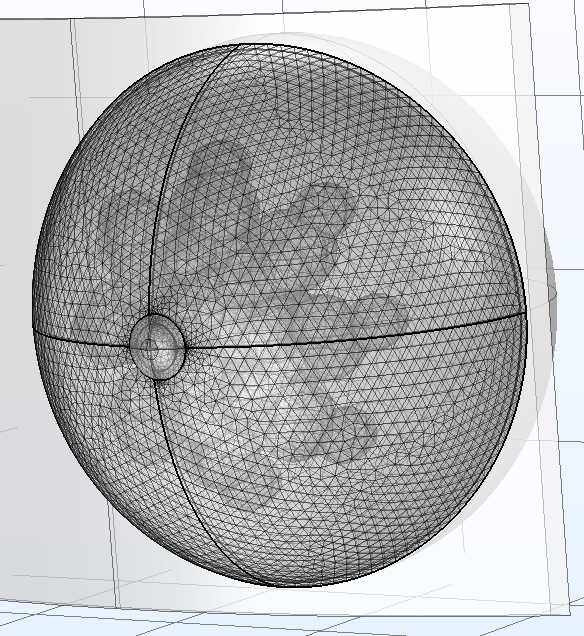
\includegraphics[width=0.45\linewidth]{Figures/M&M/report_mesh.png}
\caption{Example of the generated COMSOL tetrahedral mesh used for the breast model.}
\label{fig:comsol_mesh_example}
\end{figure}

The solver strategy consisted of a gravity-preload step followed by the time-dependent dynamic simulation. Build-only cases were used during development to verify generated selections and model setup before running full dynamic simulations.


%%%%%%%%%%%%%%%%%%%%%%%%%%%%%
% SECTION 3.6 BELOW
%%%%%%%%%%%%%%%%%%%%%%%%%%%%%


\subsection{Post-processing and evaluation metrics}
\label{post_processing_and_evaluation_metrics}

Post-processing was performed using the scripted COMSOL export and Python analysis workflow. For each completed simulation, compact output files were generated for displacement fields, selected stress quantities and time-dependent response measures. These outputs were used to evaluate how changes in model settings or parameter choices affected the simulated mechanical response, using the corresponding comparison case for each analysis.

Because the Early Warning Scan concept is based on observable breast-surface motion, the main evaluation focused on the free outer breast surface. In the COMSOL workflow this surface was represented by the \texttt{outer\_skin\_free\_bnd} selection. Whole volume displacement and stress measures were retained as supporting diagnostic quantities.

The displacement magnitude was defined as

\begin{equation}
u_{\mathrm{mag}}
=
\sqrt{u^{2}+v^{2}+w^{2}},
\label{displacement_magnitude_definition}
\end{equation}

where $u$, $v$ and $w$ are the displacement components in the $x$-, $y$- and $z$-directions. In addition to the magnitude, signed displacement components were evaluated because they preserve direction. The vertical displacement component $w$ was used to describe upward or downward surface motion during dynamic excitation.

For surface-based evaluation, spatial averages were computed over the evaluated surface selection $S$,

\begin{equation}
\bar{q}_{S}(t)
=
\frac{1}{A_{S}}
\int_{S} q(\mathbf{x},t)\,\mathrm{d}A,
\label{surface_average_metric}
\end{equation}

where $q$ is the evaluated displacement or stress quantity and $A_{S}$ is the surface area of the selection. For dynamic cases, signed vertical displacement was also evaluated relative to the dynamic-start state,

\begin{equation}
\Delta \bar{w}_{S}(t)
=
\bar{w}_{S}(t)
-
\bar{w}_{S}(t_{\mathrm{dyn,start}}).
\label{surface_vertical_displacement_from_dynamic_start}
\end{equation}

For prescribed support-displacement cases, the support-relative vertical displacement defined in Equation~\ref{support_relative_vertical_displacement} was used in addition to the absolute displacement. Landmark-patch displacements were also exported for selected surface regions, including the nipple and superior, inferior, left and right breast-surface patches. These patch-averaged values were used as robust surface-motion measures, because they are less sensitive to individual mesh nodes than single-point displacement values.

Stress was evaluated using the exported von Mises stress field. This was used as a mechanical diagnostic for comparing stress concentration between model variants. For the tumor cases, local displacement and stress measures were additionally evaluated using the tumor mask region.

COMSOL animations were also generated for qualitative inspection of the time-dependent deformation patterns. These animations were not used as quantitative evidence; the reported Results are based on the exported displacement, stress, surface and tumor-mask metrics. The post-processing quantities used for the main model comparisons are summarised in Table~\ref{post_processing_metrics_table}.

\begin{table}[H]
\centering
\small
\caption{Post-processing quantities used to compare COMSOL model variants.}
\label{post_processing_metrics_table}
\begin{tabular}{p{0.28\linewidth} p{0.32\linewidth} p{0.30\linewidth}}
\toprule
Quantity & Definition or source & Use in evaluation \\
\midrule
Free-surface displacement 
& $u$, $v$, $w$ and $u_{\mathrm{mag}}$ on \texttt{outer\_skin\_free\_bnd} 
& Main EWS-relevant surface-motion response. \\

Surface-average response 
& $\bar{q}_{S}(t)$ and $\Delta \bar{w}_{S}(t)$ 
& Average dynamic response of the visible breast surface. \\

Landmark-patch displacement 
& Patch-averaged displacement on nipple and breast-surface landmark selections 
& Robust comparison of visible local surface motion. \\

Support-relative displacement 
& $w_{\mathrm{rel}}=w-z_{\mathrm{support}}$ 
& Deformation relative to prescribed support motion. \\

von Mises stress 
& Exported COMSOL stress field 
& Mechanical stress-concentration diagnostic. \\

Tumor-region response 
& Mask-based displacement and stress measures 
& Local response around the analytic tumor overlay. \\

Peak response 
& Maximum value over the evaluated time range 
& Quantitative comparison between corresponding cases. \\
\bottomrule
\end{tabular}
\end{table}

When variants were compared, changes were reported relative to the corresponding comparison case,

\begin{equation}
\Delta q_{\%}
=
100
\frac{q_{\mathrm{variant}}-q_{\mathrm{comparison}}}{q_{\mathrm{comparison}}},
\label{relative_metric_difference}
\end{equation}

where $q$ denotes the evaluated displacement or stress metric. This percentage difference was used only when the comparison value was non-zero and physically meaningful.

%%%%%%%%%%%%%%%%%%%%%%%%%%%%%
% SECTION 3.7 BELOW
%%%%%%%%%%%%%%%%%%%%%%%%%%%%%


\subsection{Reproducibility and data management}
\label{reproducibility_and_data_management}

The project was organised to keep the COMSOL workflow reproducible and traceable. Source code, TOML case definitions, report notes and compact post-processing outputs were maintained in the project repository \cite{KuijpersEWSComsolGitHub}. Large generated files, such as full COMSOL model files, temporary solver files and extensive raw exports, were kept outside version control because they can be regenerated from the scripted case definitions.

Each COMSOL case was defined by a version-controlled TOML file. These files stored the relevant geometry route, material parameters, loading settings, mesh settings and output options for each model variant. The Python pipeline converted these case definitions into COMSOL Java builder scripts and post-processing outputs. This reduced manual editing in COMSOL and made it easier to inspect or rerun model variants.

The simulations were run using a licensed COMSOL Multiphysics installation available through TU/e. All model builds and time-dependent solves reported in this work were executed on local hardware during model development. The software and hardware environment used for the simulations is summarised in Table~\ref{software_hardware_environment_table}.

\begin{table}[H]
\centering
\small
\caption{Software and hardware environment used for COMSOL model development and simulation runs.}
\label{software_hardware_environment_table}
\begin{tabular}{p{0.32\linewidth} p{0.58\linewidth}}
\toprule
Item & Setting \\
\midrule
COMSOL version & COMSOL Multiphysics 6.4 \\
License environment & TU/e licensed COMSOL installation \\
Operating system & Windows 11 Enterprise \\
Processor & 11th Gen Intel Core i7-11800H, 2.30GHz \\
Memory & 16.0 GB RAM \\
Python environment & Python 3.8.8 \\
Repository & \cite{KuijpersEWSComsolGitHub} \\
\bottomrule
\end{tabular}
\end{table}

\newpage
\section{Results}
\label{results}

\subsection{Overview of completed model variants}
\label{overview_completed_model_variants}

% Kort: welke cases zijn succesvol gebouwd/gerund en welke vergelijking hoort bij welke route.
% Hier past een overzichtstabel met: case group, comparison case, tested variants, output status.
% Niet te veel interpretatie hier.

\subsection{Reference model response}
\label{reference_model_response}

% Hoofdresultaat van je gekozen/reference COMSOL route.
% Toon surface displacement, displacement magnitude, signed vertical displacement en von Mises stress.
% Hier past een contact sheet / surface displacement figure + compacte tabel met peak/mean metrics.

\subsection{Effect of material-parameter variation}
\label{material_parameter_sensitivity_results}

% Resultaten van stiffness/material variants.
% Denk aan no-skin/stiff/soft-interior etc.
% Focus op: surface displacement amplitude, stress response, verschil t.o.v. comparison case.
% Hier hoort je material-parameter sensitivity waar je in 3.3.2 naar verwijst.

\subsection{Effect of volumetric skin representation}
\label{volumetric_skin_results}

% Skin-enabled vs no-skin comparison.
% Vooral: skin dempt displacement, verandert stressverdeling, eventuele local stress hotspots.
% Niet opnieuw uitleggen hoe skin gemaakt is; alleen resultaten.

\subsection{Effect of Cooper-like support}
\label{cooper_support_results}

% De drie Cooper varianten: nipple--chestwall, skin-to-glandular, dense skin-to-glandular.
% Vergelijk met no-Cooper model.
% Alleen claims doen op basis van cases die echt goed gerund/gepostprocessed zijn.

\subsection{Effect of dynamic loading route}
\label{dynamic_loading_results}

% Vergelijk acceleration amplitudes en/of prescribed support displacement route.
% Focus op surface response, vertical signed motion, support-relative displacement indien relevant.
% Geen uitgebreide method uitleg meer.

\subsection{Tumor-overlay sensitivity}
\label{tumor_overlay_results}

% Tumor/no-tumor, locatie, grootte, stiffness contrast.
% Focus op EWS-relevante surface motion + lokale tumor-mask metrics.
% Hier duidelijk maken of effect globaal zichtbaar is of vooral lokaal in stress/displacement metrics.

\subsection{Summary of main result trends}
\label{summary_main_result_trends}

% Korte samenvattende tabel of bullet-like prose.
% Bijvoorbeeld: material stiffness strongest effect, skin damped motion, Cooper support route effect, tumor contrast effect.
% Geen discussie; alleen wat uit de resultaten kwam.
\newpage
\section{Discussion}
\label{discussion}

%%%%%%%%%%%%%%%%%%%%%%%%%%%%%
% SECTION 5.1 BELOW
%%%%%%%%%%%%%%%%%%%%%%%%%%%%%

\subsection{Contribution to an EWS-oriented FEM modelling workflow}
\label{discussion_ews_fem_workflow}

This project developed a progressively more complete COMSOL finite-element route for simulating dynamic breast deformation in the context of the Early Warning Scan (EWS). The main contribution was not a clinically validated detection model, but a reproducible model-development framework in which anatomical structure, material parameters, support assumptions, loading route and tumor-overlay placement can be varied in a controlled way. This distinction is important because EWS is based on observable breast-surface motion, whereas many of the model quantities used during development, such as internal stress or volume-averaged displacement, are primarily mechanical diagnostics.

Compared with a simplified breast representation, the final model route introduced a curved posterior support geometry, a more realistic glandular distribution, optional volumetric skin representation, material-parameter sensitivity cases, Cooper-like support approximations, dynamic loading variants and analytic tumor-overlay placements. These additions increased the anatomical and mechanical richness of the model and made it possible to evaluate which components most strongly affect the simulated surface response. The framework therefore provides a basis for future EWS-oriented surface-motion studies, but the present results should be interpreted as model-development outcomes rather than as evidence of diagnostic performance.


%%%%%%%%%%%%%%%%%%%%%%%%%%%%%
% SECTION 5.2 BELOW
%%%%%%%%%%%%%%%%%%%%%%%%%%%%%

\subsection{Anatomical realism and glandular representation}
\label{discussion_anatomical_realism_glandular}

A central aim of this project was to improve the anatomical realism of the FEM breast model. The realistic glandular route added a spatially distributed fibroglandular structure instead of representing the internal breast tissue with a single simplified region. This is relevant because breast deformation depends not only on total breast size, but also on the relative amount and spatial distribution of adipose and fibroglandular tissue \cite{Samani2007,Ramiao2016,Goodbrake2022,Teixeira2023}.

The current glandular implementation also introduced a practical limitation. A detailed glandular structure is mechanically more representative, but it increases geometric complexity, meshing difficulty and solver cost. Similar anatomical complexity was a limiting factor in previous internal FEBio-based model-development routes \cite{EngelsEWSReport,StormEWSReport}. The current COMSOL workflow was able to build and solve the realistic glandular route, but running many dynamic variants on a local laptop remained computationally demanding. This suggests that the modelling strategy is technically feasible, but that further studies require access to stronger computational resources.

Anatomical variability should therefore become a larger part of future model development. Breast size and shape, glandular fraction, glandular asymmetry, posterior attachment geometry and tissue distribution vary strongly between individuals \cite{Ramiao2016,Goodbrake2022,Teixeira2023}. The current model can be used as a first step for building such population-level model sets, but this would require many additional variants and more validation. Future work should therefore vary the relevant anatomical, mechanical and loading parameters in a systematic way to quantify their influence on the simulated surface response. For future AI-based analysis, this type of systematic variation could support the construction of synthetic datasets with controlled differences in anatomy, tissue properties, loading conditions and tumor characteristics.

%%%%%%%%%%%%%%%%%%%%%%%%%%%%%
% SECTION 5.3 BELOW
%%%%%%%%%%%%%%%%%%%%%%%%%%%%%

\subsection{Material-parameter uncertainty and response realism}
\label{discussion_material_uncertainty_response_realism}

Material parameters remain one of the largest sources of uncertainty in breast FEM modelling. Reported stiffness values for adipose tissue, fibroglandular tissue, skin and tumor tissue vary substantially across studies because they depend strongly on experimental protocol, tissue condition and constitutive assumptions \cite{Samani2007,Ramiao2016,Goodbrake2022,Teixeira2023}. The material settings used in this project should therefore be interpreted as controlled reference and sensitivity values rather than as patient-specific tissue properties.

This uncertainty affects how the displacement results should be read. A simulated displacement amplitude is only physically meaningful when the material parameters, boundary conditions and loading route are plausible for the intended experimental situation. The current results show that the model can produce measurable dynamic surface motion, but the exact displacement scale still requires comparison with experimental or EWS-like motion data. Such validation would make it possible to determine whether the selected stiffness range reproduces realistic breast motion.

The von Mises stress results should be interpreted with caution. In this project, von Mises stress was useful as a scalar diagnostic for comparing stress concentrations between variants, especially near support and attachment regions. However, stress is not directly measured by the EWS concept and should not be treated as a direct detection output. Stress concentrations near the posterior support are more likely to reflect the imposed boundary condition and support geometry than a clinically meaningful tissue response. For EWS interpretation, surface displacement and landmark motion are therefore more relevant than internal stress metrics.

%%%%%%%%%%%%%%%%%%%%%%%%%%%%%
% SECTION 5.4 BELOW
%%%%%%%%%%%%%%%%%%%%%%%%%%%%%

\subsection{Dynamic loading and surface-motion interpretation}
\label{discussion_dynamic_loading_surface_motion}

The dynamic loading definition is an important part of the model, because the simulated breast response depends strongly on how motion is introduced. The fixed-support acceleration input and the prescribed support-displacement route represent different idealisations of how breast motion could be generated during an EWS-like measurement. The fixed-support acceleration route applies a controlled global excitation while keeping the support geometry fixed. The prescribed support-displacement route is more directly related to a physical situation in which the chestwall or support moves up and down, for example during a jump-like motion.

In the current project, most quantitative dynamic comparisons focused on the fixed-support acceleration route. This provided a controlled way to compare model variants, but it does not necessarily mean that this route is the most realistic representation of the final EWS setup. Further work should therefore compare the fixed-support acceleration route with prescribed support-motion approaches in more detail. The resulting motion depends on the amplitude, timing, damping, gravity preload and support coupling of the model. These factors should therefore be selected or calibrated against the intended EWS motion setting, because they directly influence whether the simulated breast response is physically representative.

The current dynamic results should therefore be interpreted as proof that different loading routes can be implemented and compared within the COMSOL workflow. They do not yet define an experimentally validated EWS loading protocol. A future validation study should record the motion applied in an EWS-like setup and use that measured motion as the input or calibration target for the FEM model.

%%%%%%%%%%%%%%%%%%%%%%%%%%%%%
% SECTION 5.5 BELOW
%%%%%%%%%%%%%%%%%%%%%%%%%%%%%

\subsection{Skin and Cooper-like support modelling choices}
\label{discussion_skin_cooper_support}

The skin representation had a clear mechanical role in the model because it added a relatively stiff outer layer around the softer internal breast tissues. This is consistent with multi-component breast FEM studies, where the breast is represented using separate anatomical and mechanical components rather than as one homogeneous soft-tissue volume \cite{Chen2025,Teixeira2023,Mazier2024}. In the current COMSOL route, the $1.5~\mathrm{mm}$ volumetric skin layer was therefore an important step toward a more anatomically representative model. This thickness is also within reported breast-skin thickness ranges, although skin thickness and mechanical properties vary between subjects and measurement locations \cite{Huang2008,Sutradhar2012}.

The volumetric skin route should still be interpreted as a controlled modelling choice rather than as a patient-specific skin reconstruction. Its mechanical effect depends not only on the selected skin stiffness and thickness, but also on how the layer is coupled to the internal breast tissue. Future work should therefore include a more systematic skin-parameter study to determine how robust the simulated surface response is across realistic skin properties.

The Cooper-like support implementation should also be interpreted as an approximation. Cooper's ligaments form a distributed fibrous support structure in the breast, while the current COMSOL route represented their influence through simplified support terms rather than explicit anatomical ligament reconstruction \cite{Chen2025}. This made it possible to test the mechanical influence of additional support, but future versions should use a more anatomically support representation for the Cooper's ligaments.

%%%%%%%%%%%%%%%%%%%%%%%%%%%%%
% SECTION 5.6 BELOW
%%%%%%%%%%%%%%%%%%%%%%%%%%%%%

\subsection{Tumor-overlay route and future tumor sensitivity}
\label{discussion_tumor_overlay_future_sensitivity}

The tumor-overlay route successfully added a build-level mechanism for placing analytic spherical stiffness inclusions inside the existing breast volume. This is a useful first step because tumor size and location can be changed without rebuilding the full breast geometry for every variant. The current implementation is therefore suitable for preparing systematic tumor-sensitivity studies.

The current tumor representation is still simplified. Real breast tumors can differ in morphology, stiffness, depth and interaction with surrounding tissue, and reported tumor stiffness values vary strongly between measurement methods and tumor types \cite{Samani2007,McKnight2002,Patel2021,Patel2022}. A spherical homogeneous overlay can test the effect of a controlled stiffness contrast, but it cannot represent the full range of malignant tumor morphology. This limitation is especially important for EWS, because a tumor would only be detectable through its effect on the externally observable surface motion. The relevant question is therefore not only whether a stiff inclusion changes the internal mechanical field, but whether it changes the surface response enough to be measured robustly.

Future tumor studies should therefore test a broader range of tumor geometries, stiffness contrasts and anatomical locations. These studies should be run as complete dynamic simulations with tumor-mask post-processing, surface-motion metrics and matched no-tumor controls. Only after such a solved and validated case set is available can the tumor-overlay route be used to discuss potential EWS detectability.

%%%%%%%%%%%%%%%%%%%%%%%%%%%%%
% SECTION 5.7 BELOW
%%%%%%%%%%%%%%%%%%%%%%%%%%%%%

\subsection{Computational limitations and reproducibility}
\label{discussion_computational_limitations_reproducibility}

A major limitation of the current project was that all COMSOL model builds and time-dependent simulations were run on a personal laptop. This was workable for developing the pipeline and generating geometry build-only cases, but it strongly limited the number of complete dynamic solves that could be included. For the more realistic model variants, individual dynamic simulations could take approximately $12~\mathrm{h}$ per case, not including the additional time required for post-processing. This made large parameter sweeps and complete dynamic testing of the more complex model routes impractical within the project timeframe.

Access to faster external computational resources would improve the study by allowing larger sweeps, more realistic model variants and full post-processing to be run more efficiently. This would be especially important for systematic testing of material parameters, dynamic loading routes, Cooper-like support and tumor-overlay cases. The current computational limitation should therefore be interpreted as a practical limitation of the project setup and timeframe, rather than as a limitation of the modelling framework itself. Future work should account for this by running the simulations on stronger computational hardware.

The repository structure helped keep the model-development workflow traceable. The scripted case definitions, compact outputs, report notes and figure sources made it possible to track how the model variants were generated and evaluated \cite{KuijpersEWSComsolGitHub}. Future work should keep this level of traceability, especially when larger simulation sets are generated on external computational resources.


%%%%%%%%%%%%%%%%%%%%%%%%%%%%%
% SECTION 5.8 BELOW
%%%%%%%%%%%%%%%%%%%%%%%%%%%%%

\subsection{Overall perspective and future work}
\label{discussion_overall_perspective_future_work}

Overall, the project extended the COMSOL FEM breast model in several directions that are relevant for future EWS-oriented deformation studies:

\begin{itemize}
    \item a more anatomically detailed breast geometry with chestwall curvature, asymmetry options and a realistic glandular tissue distribution;
    \item controlled material-parameter and volumetric-skin variants;
    \item simplified Cooper-like support and dynamic loading routes;
    \item analytic tumor-overlay placement for future stiffness-sensitivity studies;
    \item a traceable workflow for case definition, model building and automatic post-processing.
\end{itemize}

The most important next step is to run systematic, fully solved dynamic simulations on stronger computational hardware and compare the simulated surface response with experimental or EWS-like measurement data. This should be combined with controlled variation of material parameters, glandular anatomy, skin properties, loading route and tumor properties. If those future simulations show that tumor-related stiffness contrasts produce measurable and repeatable differences in breast-surface motion, the model could become a useful tool for exploring EWS sensitivity and design choices.


\newpage
\section{Conclusion}

This project developed a reproducible COMSOL finite-element workflow for EWS-oriented breast deformation modelling. The final workflow supports controlled variation of anatomical geometry, tissue distribution, material parameters, skin representation, support assumptions, loading route and tumor-overlay placement.

The strongest quantitative effects were found for the material and skin-parameter variants. Volumetric skin representation and skin stiffness had a large influence on peak displacement and local von Mises stress concentrations. In contrast, the simplified Cooper-like support variants produced only small global displacement changes in the available scout results, so they should be interpreted as support-sensitivity implementation checks rather than as validated anatomical ligament models.

The tumor-overlay route was implemented at build level and visualised for different tumor sizes and locations. This confirms that analytic spherical tumor masks can be placed inside the anatomical breast model, but it does not yet provide quantitative evidence for tumor detectability. Complete tumor-sensitivity studies require matched no-tumor controls, fully solved dynamic cases, surface-based post-processing and validation against experimental or EWS-like surface-motion data. Overall, the project provides a traceable COMSOL FEM platform for future EWS model development, while showing that stronger computational resources are needed for systematic large-scale simulation and validation.
% \newpage
% \section{AI-tools}
% Wanneer nodig, vermelden % Wanneer nodig vermelden
\newpage
\bibliographystyle{IEEEtran}
\bibliography{references.bib}
\newpage
\addcontentsline{toc}{section}{Appendix}
\addtocontents{toc}{\protect\setcounter{tocdepth}{0}}
\appendix

\clearpage
\section*{Appendix}
\addcontentsline{toc}{section}{Appendix}

\section{Previous EWS FEM work}
\label{sec:appendix_previous_ews_fem_work}

The present project was developed in the context of previous internal Early Warning Scan (EWS) finite element modelling work. Earlier EWS models provided a methodological starting point for parametrised breast geometry, soft-tissue material assumptions, dynamic loading and displacement-based evaluation \cite{EngelsEWSReport, StormEWSReport}. These previous projects were used as internal engineering reference material and as a comparison point for modelling choices. They were not used as validation datasets for the current COMSOL model.

The earlier FEBio-oriented modelling route used a simplified parametrised breast representation in which adipose and glandular regions were defined from geometric construction parameters. Figure~\ref{fig:appendix_previous_ews_cross_section} shows a schematic cross-section from the earlier EWS project by R. Engels \cite{EngelsEWSReport}. This representation provided useful context for the transition toward a COMSOL-based workflow, but the current COMSOL model does not reproduce the previous geometry directly.

\begin{figure}[H]
\centering
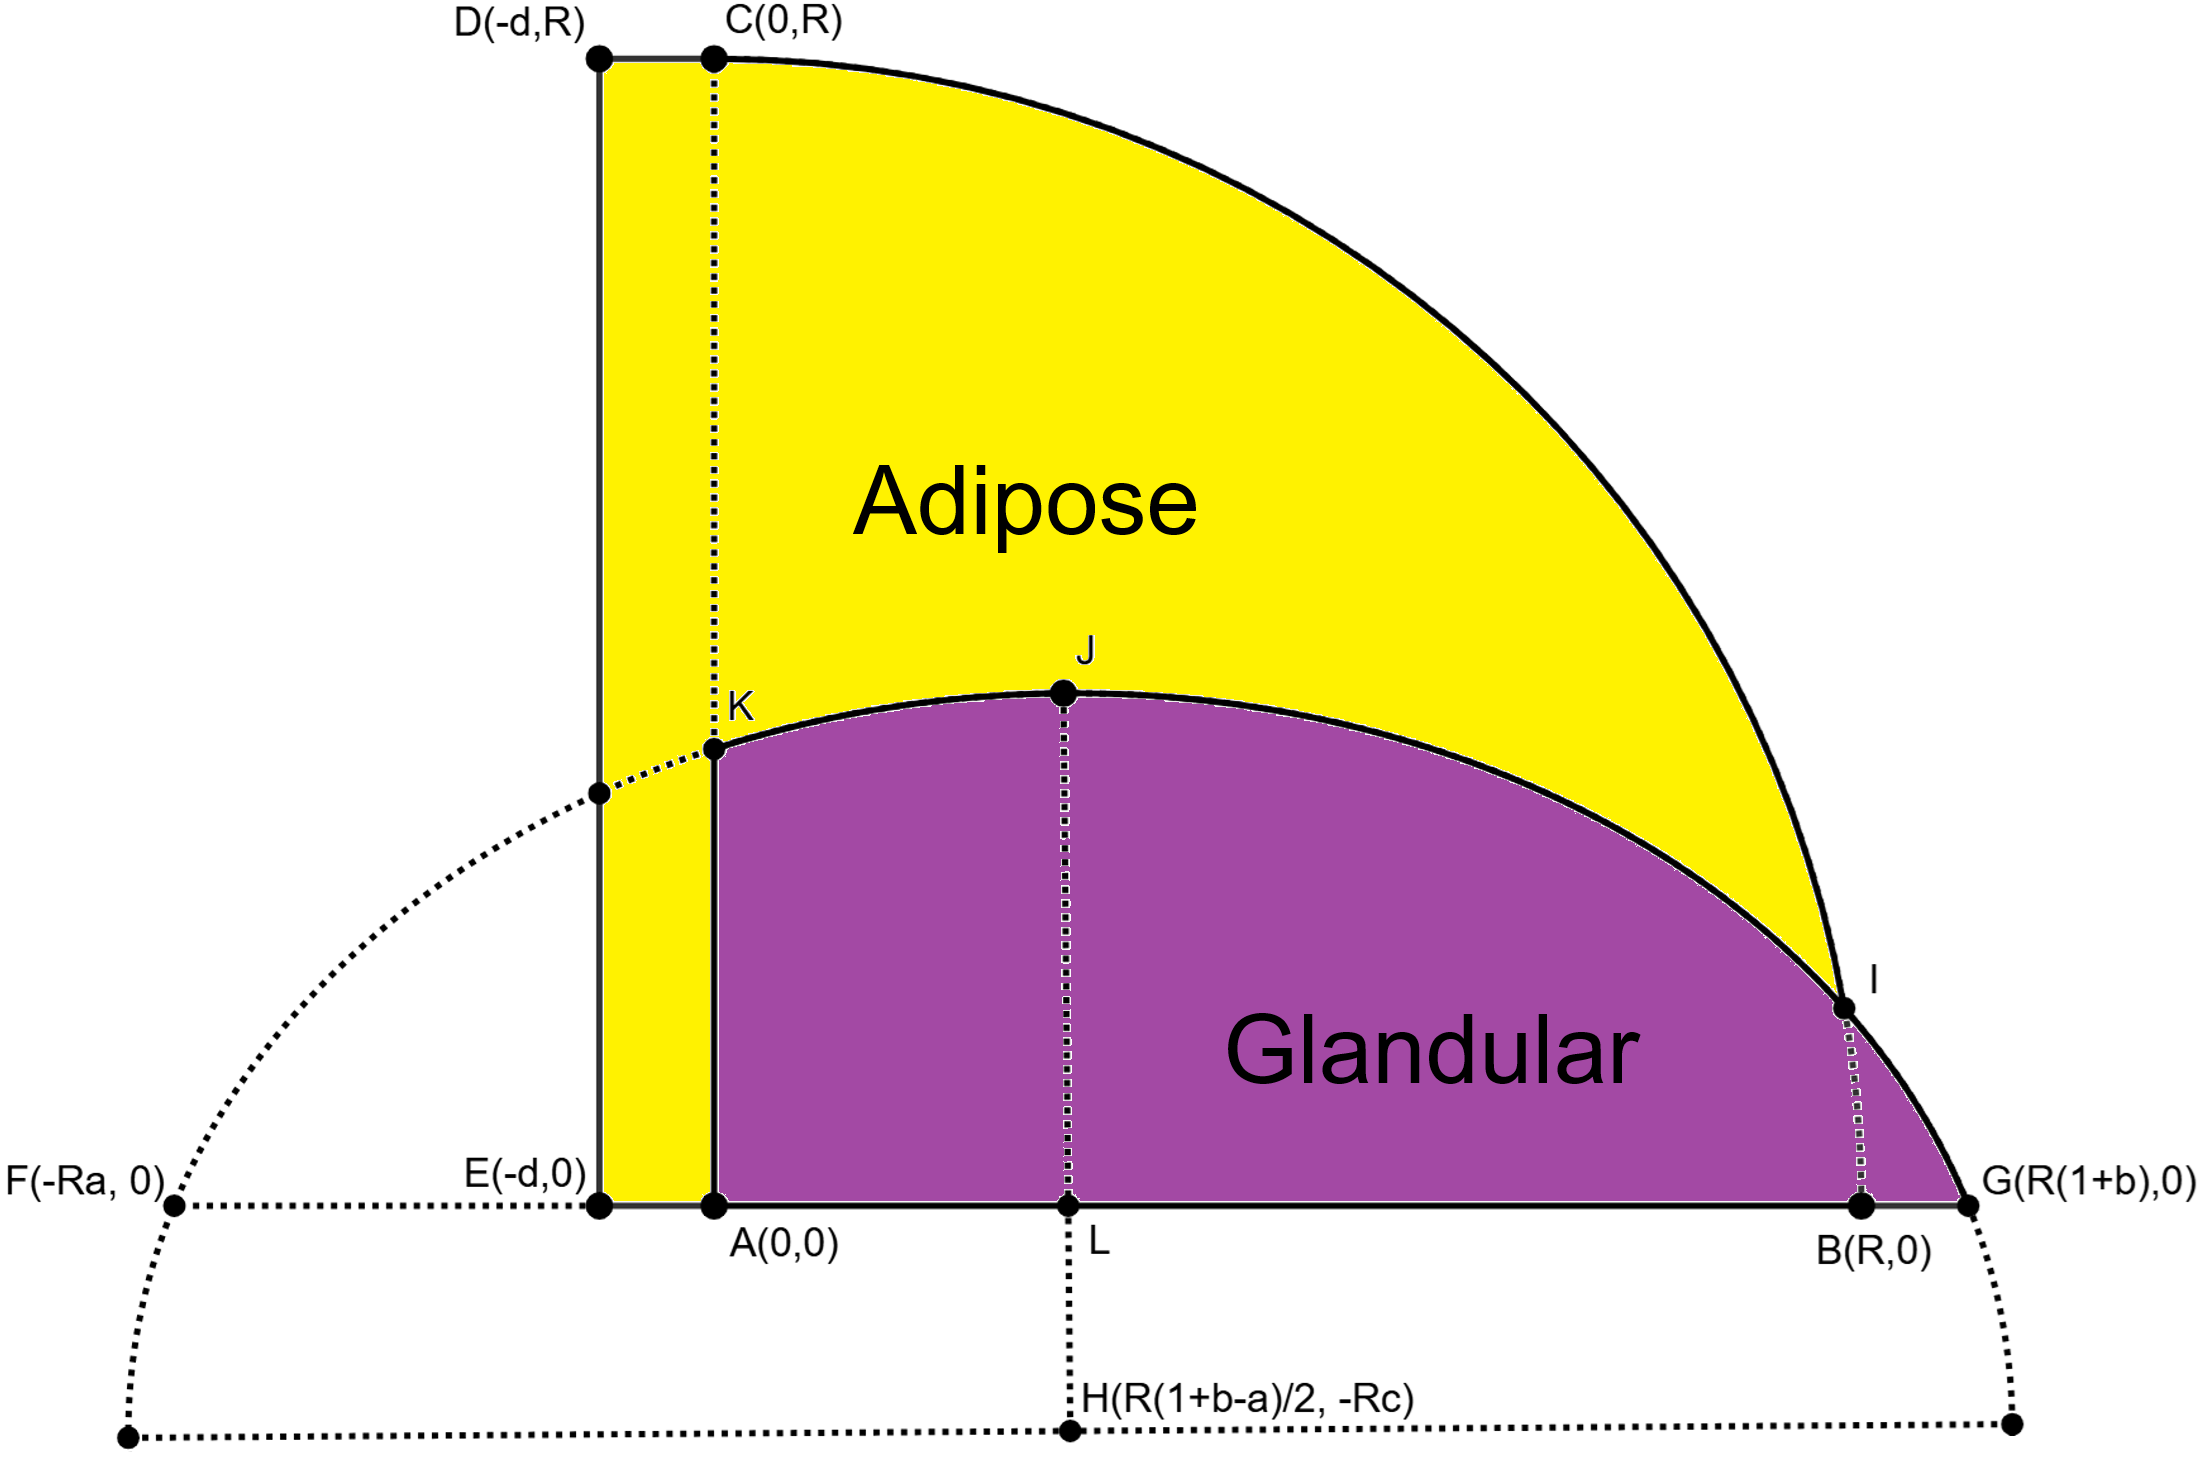
\includegraphics[width=0.85\linewidth]{Figures/Appendix/breast_crossesction.png}
\caption{Schematic cross-section from the earlier EWS FEM breast model by R. Engels \cite{EngelsEWSReport}. The figure illustrates the parametrised adipose and glandular regions used in that previous modelling route and is included here as internal methodological context.}
\label{fig:appendix_previous_ews_cross_section}
\end{figure}

The later EWS/SIOUX workflow provided additional context for skin representation, soft material settings and distributed reinforcement concepts for Cooper-ligament-like support \cite{StormEWSReport}. In the current project, these earlier modelling choices were treated as reference points rather than as fixed requirements. The COMSOL route was developed as a separate implementation with emphasis on controlled geometry construction, automated region definitions, build-only checks and systematic comparison between model variants. This made it possible to investigate selected anatomical and mechanical modelling assumptions in a more traceable way, without implying that the current model is a validated patient-specific representation.

\newpage
\section{Current COMSOL repository and reproducibility structure}
\label{sec:appendix_current_repository}

The active implementation used in this internship project is the COMSOL source-case pipeline developed during this project. The public project repository stores the reproducible parts of the work, including the Python source code, active TOML case definitions, report notes, plotting scripts, compact post-processing tables and selected figures \cite{KuijpersEWSComsolGitHub}. Large generated COMSOL files, build folders, solve folders, recovery files and raw exports are not intended to be stored in the repository because they can become several gigabytes per case.

The main repository folders used for the current COMSOL workflow are summarised in Table~\ref{tab:appendix_repository_structure}. The exact folder structure may still change during repository cleanup, but the distinction between source definitions, generated artefacts and compact evaluation output was maintained throughout the project.

\begin{table}[H]
\centering
\caption{Main repository components used in the COMSOL model-development workflow.}
\label{tab:appendix_repository_structure}
\begin{tabular}{p{0.40\linewidth} p{0.50\linewidth}}
\toprule
Repository component & Role in the project \\
\midrule
\texttt{src/ews\_fem\_pipeline\_comsol} & Active Python package for the COMSOL source-case workflow, including case loading, model generation support, Java builder generation, run control and post-processing utilities. \\
\texttt{runs/comsol\_runs} & Version-controlled TOML case definitions for the main model variants and sensitivity studies. \\
\texttt{analysis\_output/comsol\_pipeline} & Compact evaluation outputs used for comparison, including summary tables, selected plots and post-processing results. \\
\texttt{docs/report\_notes/comsol\_pipeline} & Project notes documenting modelling choices, run status, figure sources and interpretation decisions. \\
\texttt{docs/Internship\_report\_Daan\_Kuijpers} & The final intership project report. \\
\bottomrule
\end{tabular}
\end{table}

The COMSOL simulations were run using a licensed COMSOL Multiphysics installation available through TU/e. Most model builds and dynamic solves were executed on local hardware during model development. Because time-dependent COMSOL solves can be computationally expensive, especially for second-order elements, volumetric skin layers and larger parameter sweeps, access to stronger computational resources such as TU/e high-performance computing facilities is relevant for future large-scale studies. In this project, the repository was therefore organised to preserve the reproducible case definitions and compact outputs, while allowing heavy generated artefacts to remain outside version control.

\newpage
\section{Simplified example of a COMSOL case definition}
\label{sec:appendix_example_case_definition}

The COMSOL pipeline uses TOML case definitions to specify the main model settings. The full case files contain more detailed options than shown below. Listing~\ref{lst:appendix_simplified_toml} gives a simplified example to illustrate how geometry, material, loading and evaluation settings are defined in a traceable format.

\begin{lstlisting}[
caption={Simplified example of a COMSOL case definition. Only the main settings are shown; the complete case definitions are stored in the project repository.},
label={lst:appendix_simplified_toml}
]
[case]
name = "example_reference_case"
description = "Simplified reference case for documentation"

[geometry]
breast_volume_ml = 585
chestwall_variant = "xoffset055"
glandular_distribution = "realistic_reference"
outer_shape_asymmetry = "none"

[materials]
adipose_set = "reference"
glandular_set = "reference"
skin_layer = "none"
cooper_support = "none"

[loading]
type = "fixed_support_acceleration"
amplitude_g = 0.25
duration_s = 0.60
mass_damping_alpha = 60

[tumor]
enabled = false

[evaluation]
export_displacement = true
export_von_mises_stress = true
export_surface_metrics = true
\end{lstlisting}

The purpose of these case definitions is not only to automate COMSOL runs, but also to make the modelling assumptions explicit. When a model variant is changed, the corresponding TOML file records which geometry, material, loading or evaluation setting was modified. This makes comparisons between model variants more transparent than manually editing a single COMSOL model file for each simulation.

\newpage
\section{Breast-volume reference data}
\label{sec:appendix_breast_volume_reference}

An internal Catharina Hospital breast-volume dataset was reviewed to contextualise the selected COMSOL reference volume. The dataset consisted of 100 manually delineated breast volumes. The contours were drawn approximately 5~mm inside the outer skin boundary on images acquired in a supine position. The reported values should therefore be interpreted as internal reference volumes for model scaling, rather than as exact external breast volumes.

\begin{table}[H]
\centering
\caption{Summary of the internal Catharina Hospital breast-volume reference dataset. The dataset contained 100 manually delineated breast volumes, with contours drawn approximately 5~mm inside the outer skin boundary in supine images.}
\label{tab:appendix_breast_volume_reference}
\begin{tabular}{lc}
\toprule
Metric & Breast volume (mL) \\
\midrule
Mean & 728.32 \\
Median & 691.15 \\
Standard deviation & 327.39 \\
25th percentile & 519.65 \\
75th percentile & 928.70 \\
Minimum & 105.68 \\
Maximum & 1777.28 \\
\bottomrule
\end{tabular}
\end{table}

The selected COMSOL reference volume of $\sim$585~mL lies between the 25th percentile and the median of this internal dataset. This supports its use as a lower-mid reference volume for the current model-development route. Direct comparison remains limited by the segmentation definition and patient position, because the internal contours were drawn inside the skin boundary and in a supine position.

The internal dataset was also compared with literature values for breast-volume measurement. Stahl et al. reported MRI-based breast anthropometry in a cohort of 400 women and showed a broad distribution of breast volumes \cite{Stahl2023}. Yoo et al. compared MRI-estimated breast volume with mastectomy specimen weight and supports the clinical relevance of MRI-based volume estimation, although in a cancer/mastectomy cohort \cite{Yoo2013}. Nie et al. showed that skin removal can change quantitative MRI-based breast-volume and density measurements, which is relevant because the internal dataset was delineated inside the outer skin boundary \cite{Nie2010SkinRemoval}. Choppin et al. reviewed breast-volume measurement methods and emphasised that measurement uncertainty depends strongly on method, patient pose and boundary definition \cite{Choppin2016}. Together, these sources support using the $\sim$585~mL COMSOL volume as a defensible controlled reference volume, while avoiding overinterpretation as an exact population average.

\newpage
\section{Fibroglandular fraction reference data}
\label{sec:appendix_glandular_fraction_reference}

The selected Stage~3 reference model was compared with literature on volumetric breast density and fibroglandular tissue quantification. This comparison was used to contextualise the chosen fibroglandular fraction, not to assign a clinical BI-RADS category to the model.

\begin{table}[H]
\centering
\caption{Literature context used to interpret the selected fibroglandular fraction. The model fraction refers to three-dimensional fibroglandular volume divided by total breast volume.}
\label{tab:appendix_glandular_fraction_reference}
\begin{tabular}{p{0.30\linewidth} p{0.58\linewidth}}
\toprule
Source & Relevance for this model \\
\midrule
Sartor et al. \cite{Sartor2016} & Compares qualitative radiologist density classification with automated volumetric assessment and provides context for volumetric density groups. \\
Nie et al. \cite{Nie2010} & Quantifies three-dimensional fibroglandular tissue patterns from MRI and reports volumetric breast and fibroglandular tissue measurements. \\
Lu et al. \cite{Lu2012} & Compares breast tissue measurements across MRI, mammography and mathematical estimation, and shows that individual fibroglandular fractions can vary substantially. \\
ACR BI-RADS \cite{ACRBIRADS} & Provides the clinical breast-composition framework, but these categories are not directly equivalent to the model's three-dimensional fibroglandular volume fraction. \\
\bottomrule
\end{tabular}
\end{table}

This density context is also relevant for the EWS application. Women with dense breasts are more difficult to screen using X-ray mammography because fibroglandular tissue can reduce lesion conspicuity and lower mammographic sensitivity \cite{VonEuler-Chelpin2019,Bakker2019}. For this reason, a relatively fibroglandular-rich reference model is useful for EWS-oriented model development, provided that it is not interpreted as a population-average breast composition.

The selected COMSOL reference case produced a breast volume of approximately 585~mL and a glandular fraction of 24.308\%, corresponding to an approximate glandular volume of 142.2~mL. This value is higher than typical average volumetric density values reported in screening populations, but remains defensible as a controlled fibroglandular-rich reference for EWS-oriented model development. It should therefore be interpreted as a selected anatomical reference configuration rather than as a population-average breast-density value or a direct BI-RADS category.

\newpage
\section{Material-parameter literature summary}
\label{appendix_material_parameter_literature_summary}

The material parameters used in the COMSOL model were selected as controlled reference and sensitivity values rather than as patient-specific tissue measurements. Reported breast-tissue stiffness values vary strongly between studies because they depend on measurement protocol, tissue preparation, preload, strain level, loading direction, subject characteristics and constitutive model \cite{Samani2007,Ramiao2016,Goodbrake2022,Teixeira2023}. The literature was therefore used to define plausible stiffness scales and sensitivity ranges, not to identify one unique material parameter set.

\begin{table}[H]
\centering
\small
\caption{Summary of the literature-based rationale used for selecting the material-parameter scales in the COMSOL model.}
\label{appendix_material_parameter_rationale_table}
\begin{tabular}{p{0.20\linewidth} p{0.34\linewidth} p{0.36\linewidth}}
\toprule
Model component & Literature interpretation & Use in the COMSOL model \\
\midrule
Adipose tissue 
& Normal breast adipose tissue is generally reported in the low-kPa stiffness range, although values differ between ex-vivo testing, elastography and model calibration studies \cite{Samani2007,Ramiao2016,Teixeira2023}. 
& The reference adipose material was assigned an approximate small-strain stiffness of $E\approx3.66~\mathrm{kPa}$. Softer and intermediate variants were included as material-stiffness sensitivity cases. \\

Fibroglandular tissue 
& Fibroglandular tissue is typically stiffer and more heterogeneous than adipose tissue. Three-dimensional testing also indicates that human breast tissue can show direction-dependent and spatially heterogeneous behaviour \cite{Goodbrake2022}. 
& The reference fibroglandular material was assigned an approximate small-strain stiffness of $E\approx10~\mathrm{kPa}$. Additional variants were used to test the sensitivity of the simulated response to internal tissue stiffness. \\

Skin layer 
& Skin is mechanically relevant in breast deformation models and is commonly represented as a stiffer component than the internal breast tissues. Its effective contribution depends on both material stiffness and layer thickness \cite{Chen2025,Teixeira2023}. 
& The active volumetric-skin route used a thickness of $1.5~\mathrm{mm}$ and an approximate stiffness scale of $E\approx500~\mathrm{kPa}$. Lower skin-stiffness cases were retained only as sensitivity variants. \\

Tumor overlay 
& Tumor tissue is generally reported to be stiffer than surrounding normal tissue, but the reported stiffness range depends strongly on imaging modality, tissue type and region of interest \cite{Samani2007,McKnight2002,Patel2021,Patel2022}. 
& The hard tumor-overlay setting targeted an approximate stiffness scale of $E\approx100~\mathrm{kPa}$. This value was used to create a clear stiffness contrast, not as a patient-specific tumor calibration. \\

Posterior support 
& The posterior thoracic region was not modelled as a detailed anatomical chest wall. Instead, it was included as a simplified mechanical support region for the breast model. 
& The constructed posterior support domain was assigned a linear elastic surrogate material with $E=10~\mathrm{kPa}$ and $\nu=0.49$. \\
\bottomrule
\end{tabular}
\end{table}

Overall, the selected parameters should be interpreted as a controlled modelling set for comparing material routes and sensitivity cases. The values define consistent stiffness scales for the COMSOL workflow, while acknowledging that breast tissue, skin and tumor properties cannot be represented by a single universally accepted parameter value.





%%%%%%%%%%%%%%%%%%%%%%%%%%%%% eruit of veranderen appendix hieronder
\newpage
\section{Figure and metric sources}
\label{sec:appendix_figure_metric_sources}

The figures and quantitative values in the main report are based on selected COMSOL outputs, compact post-processing files and generated plots. The complete figure and metric source index is stored in \texttt{docs/report\_notes/comsol\_pipeline/report\_figures\_metrics\_index.md}. This index records the relevant COMSOL output folders, metric files and source images used to create the report figures.

The appendix figures below are included as provenance material. They document the source contact sheets and geometry screenshots used during model development. They are not all intended to carry the same quantitative interpretation as the main results.

\begin{figure}[H]
\centering
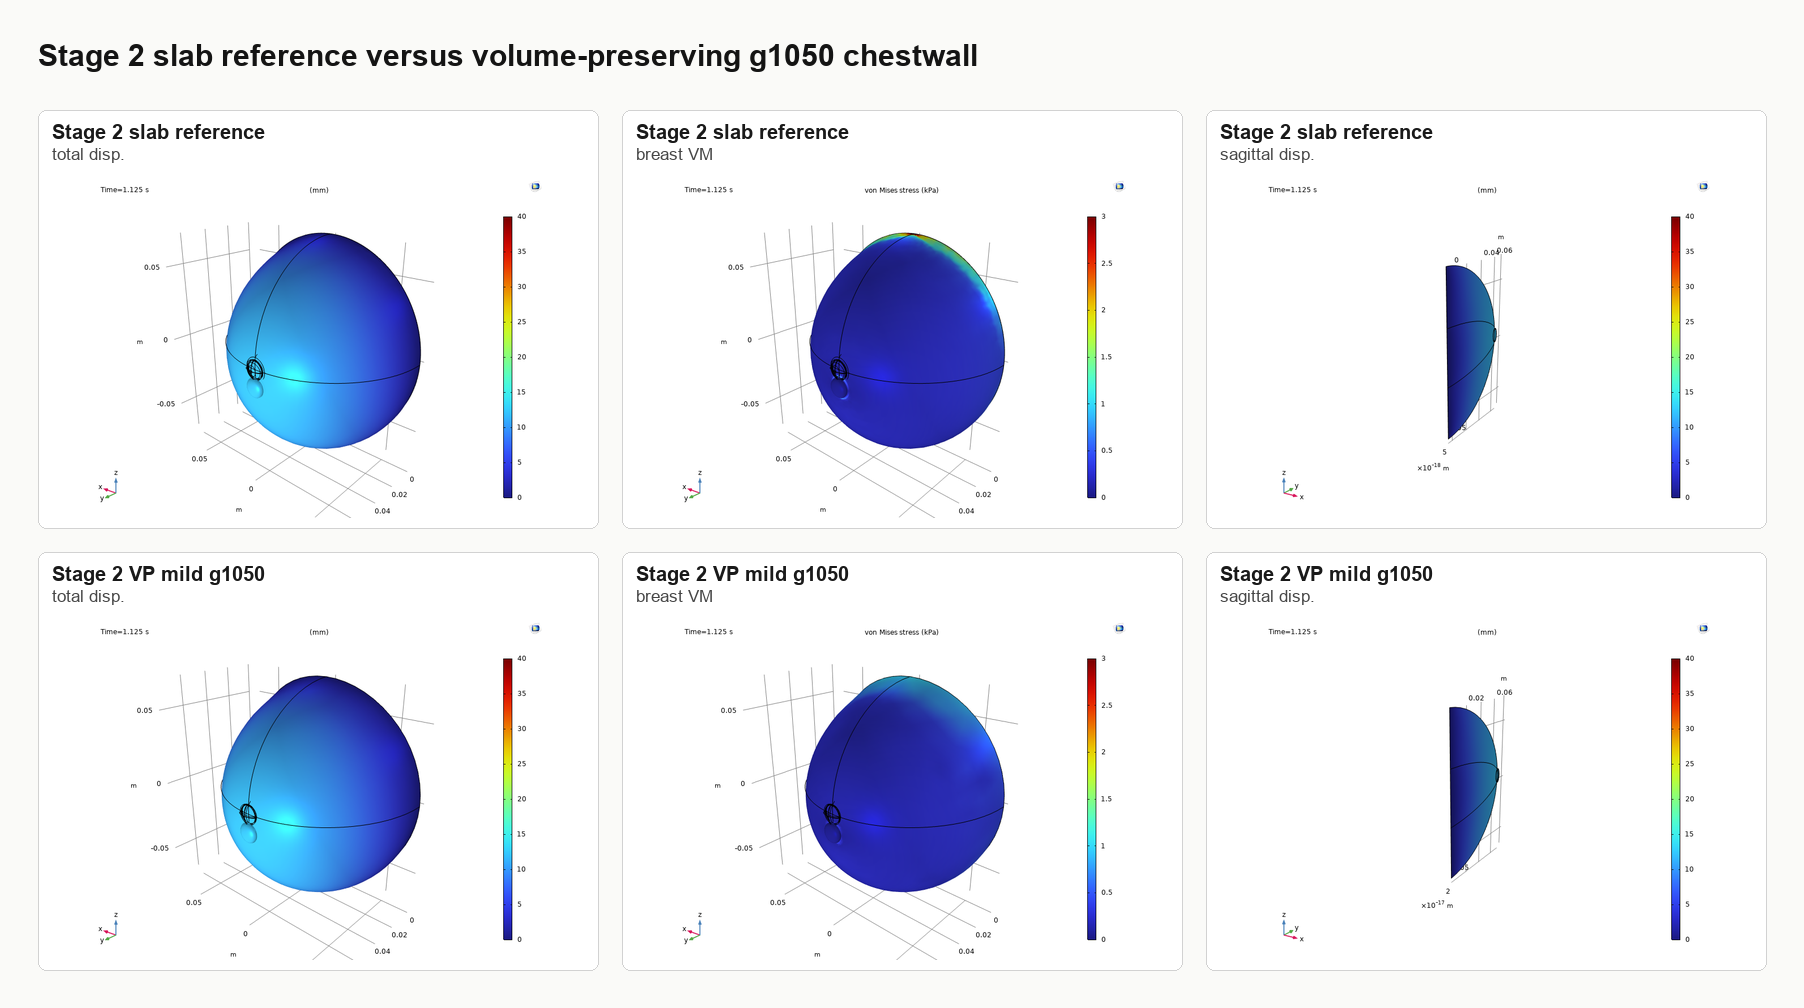
\includegraphics[width=0.95\linewidth,height=0.78\textheight,keepaspectratio]{Figures/comsol_contact_sheets/stage2_chestwall_contact_sheet.png}
\caption{Source contact sheet for the selected chestwall-geometry route. The figure documents displacement and von Mises stress panels used during the evaluation of the curved posterior support geometry.}
\label{fig:appendix_stage2_figures}
\end{figure}

\begin{figure}[H]
\centering
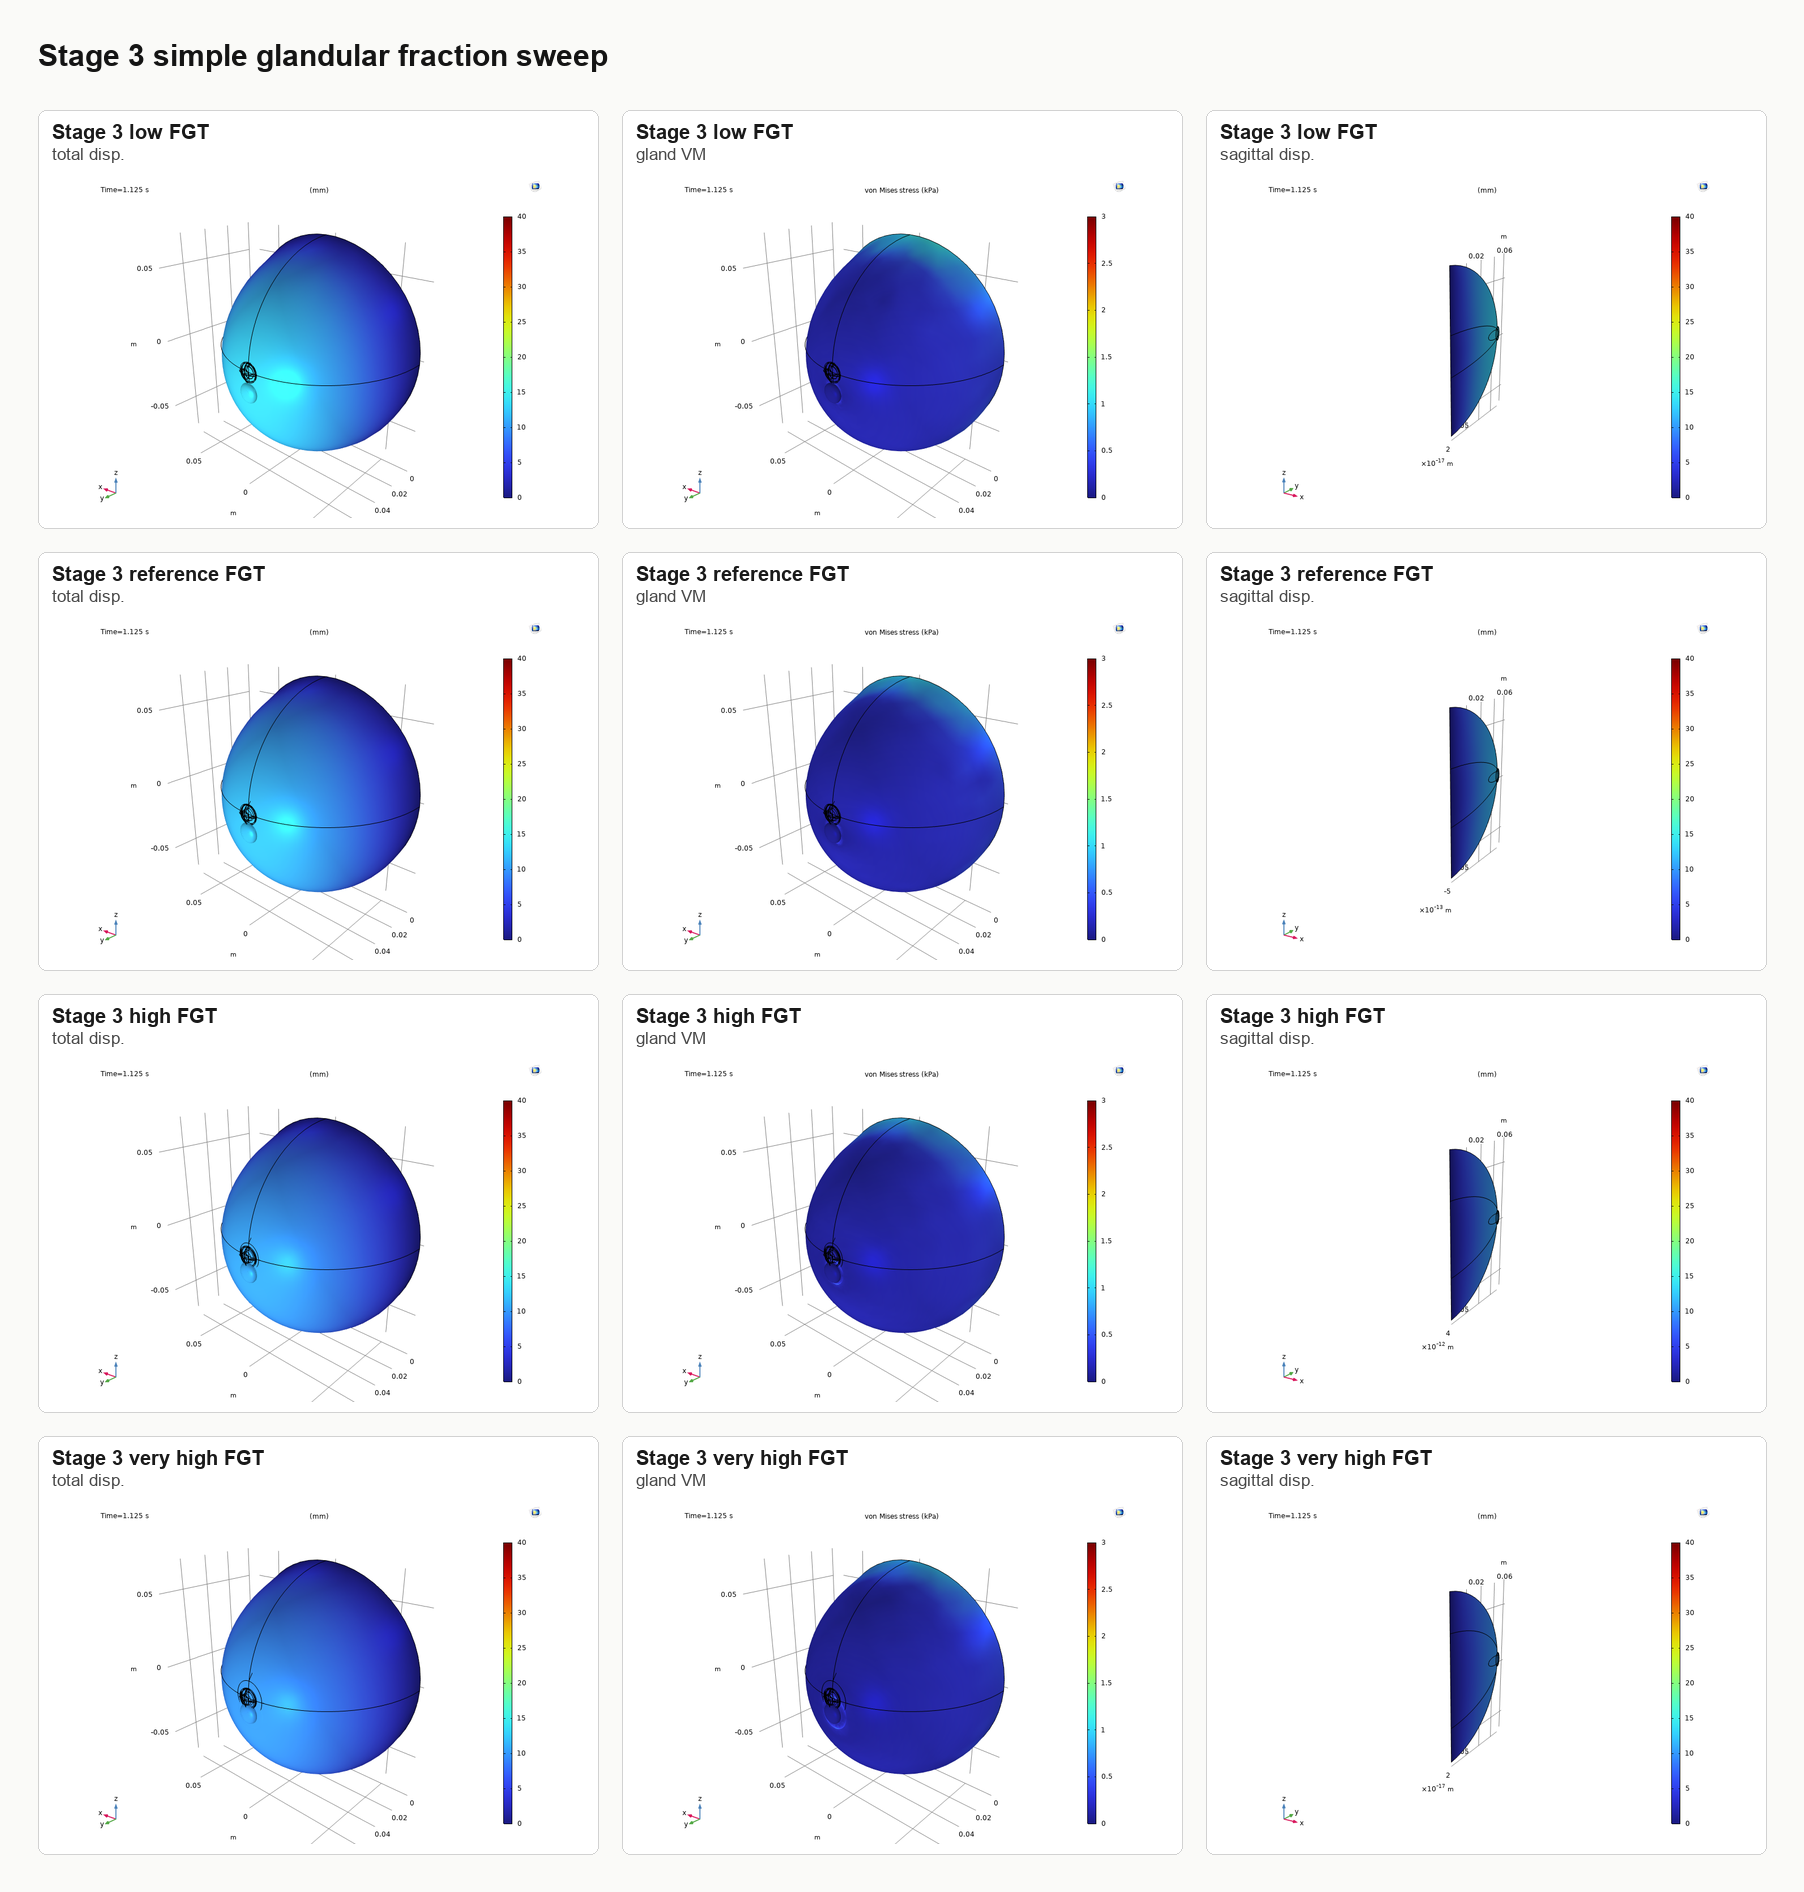
\includegraphics[width=0.95\linewidth,height=0.78\textheight,keepaspectratio]{Figures/comsol_contact_sheets/stage3_glandular_fraction_contact_sheet.png}
\caption{Source contact sheet for the glandular-distribution comparison. The figure documents the solved simple glandular fraction sensitivity and supports the transition toward a more realistic glandular reference.}
\label{fig:appendix_stage3_fraction_figures}
\end{figure}

\begin{figure}[H]
\centering
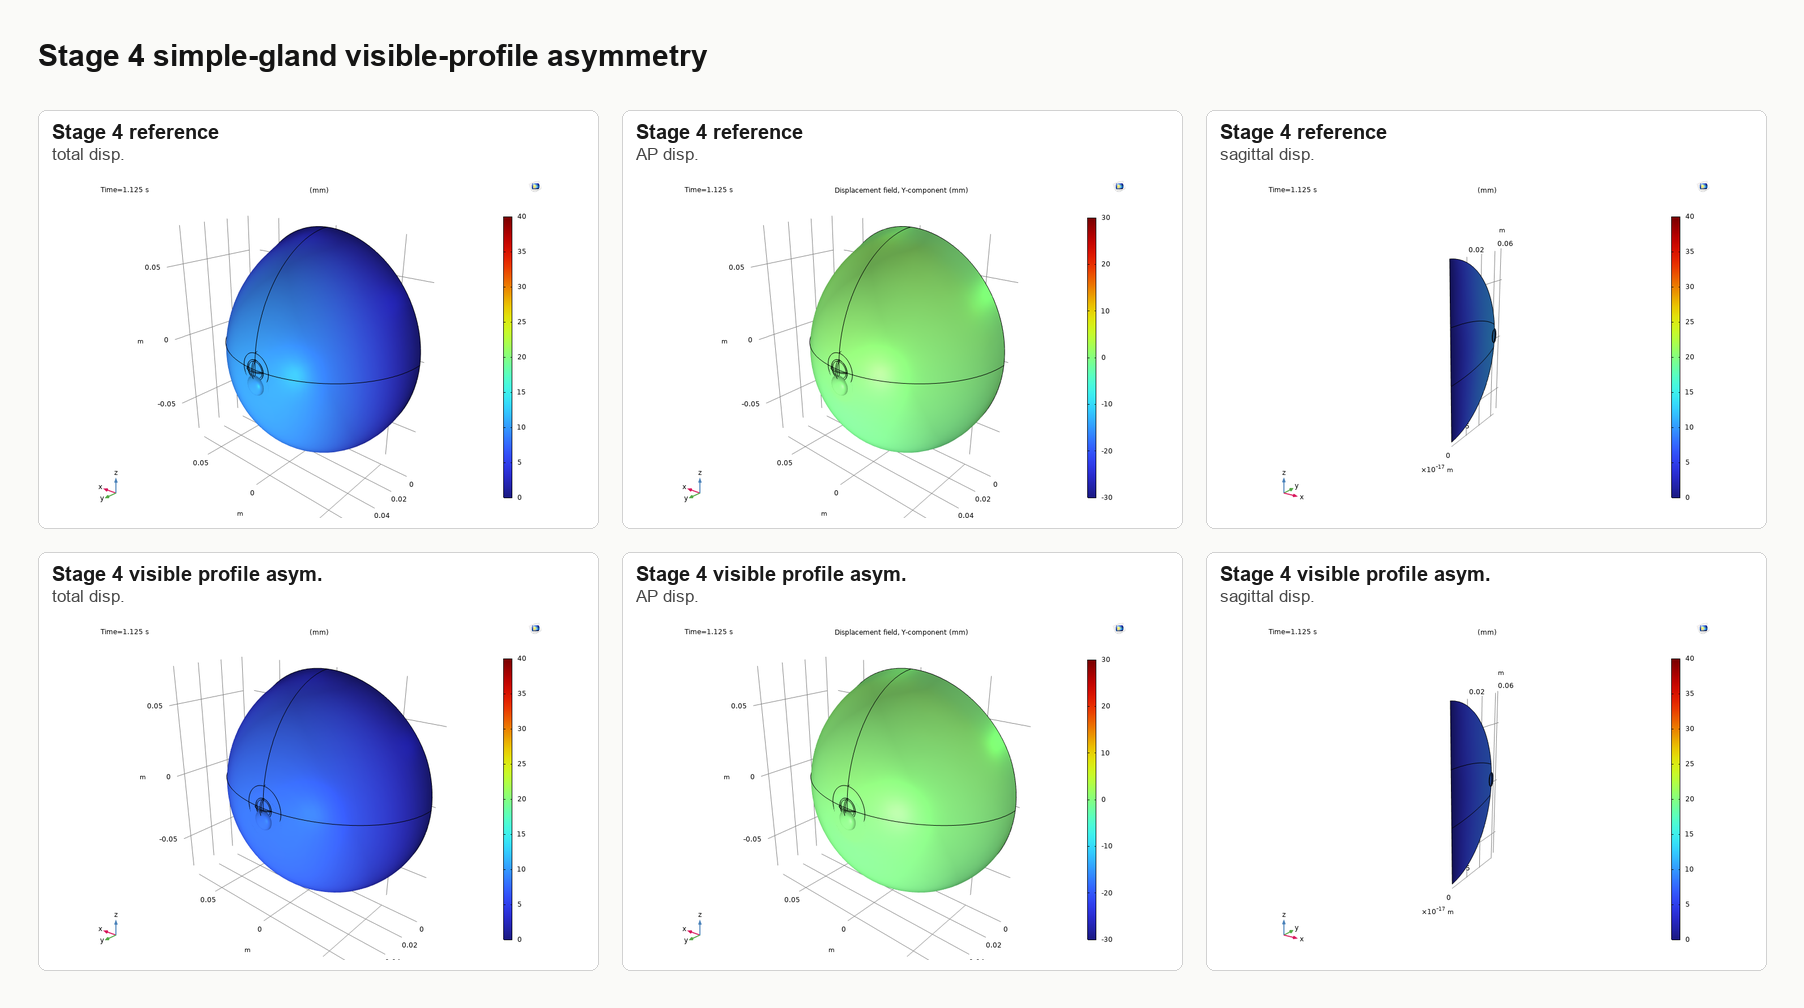
\includegraphics[width=0.95\linewidth,height=0.78\textheight,keepaspectratio]{Figures/comsol_contact_sheets/stage4_asymmetry_contact_sheet.png}
\caption{Source contact sheet for outer-shape and nipple-position sensitivity checks. These cases are used as geometry-development context and should be interpreted separately from the matched reference comparisons.}
\label{fig:appendix_stage4_figures}
\end{figure}

\begin{figure}[H]
\centering
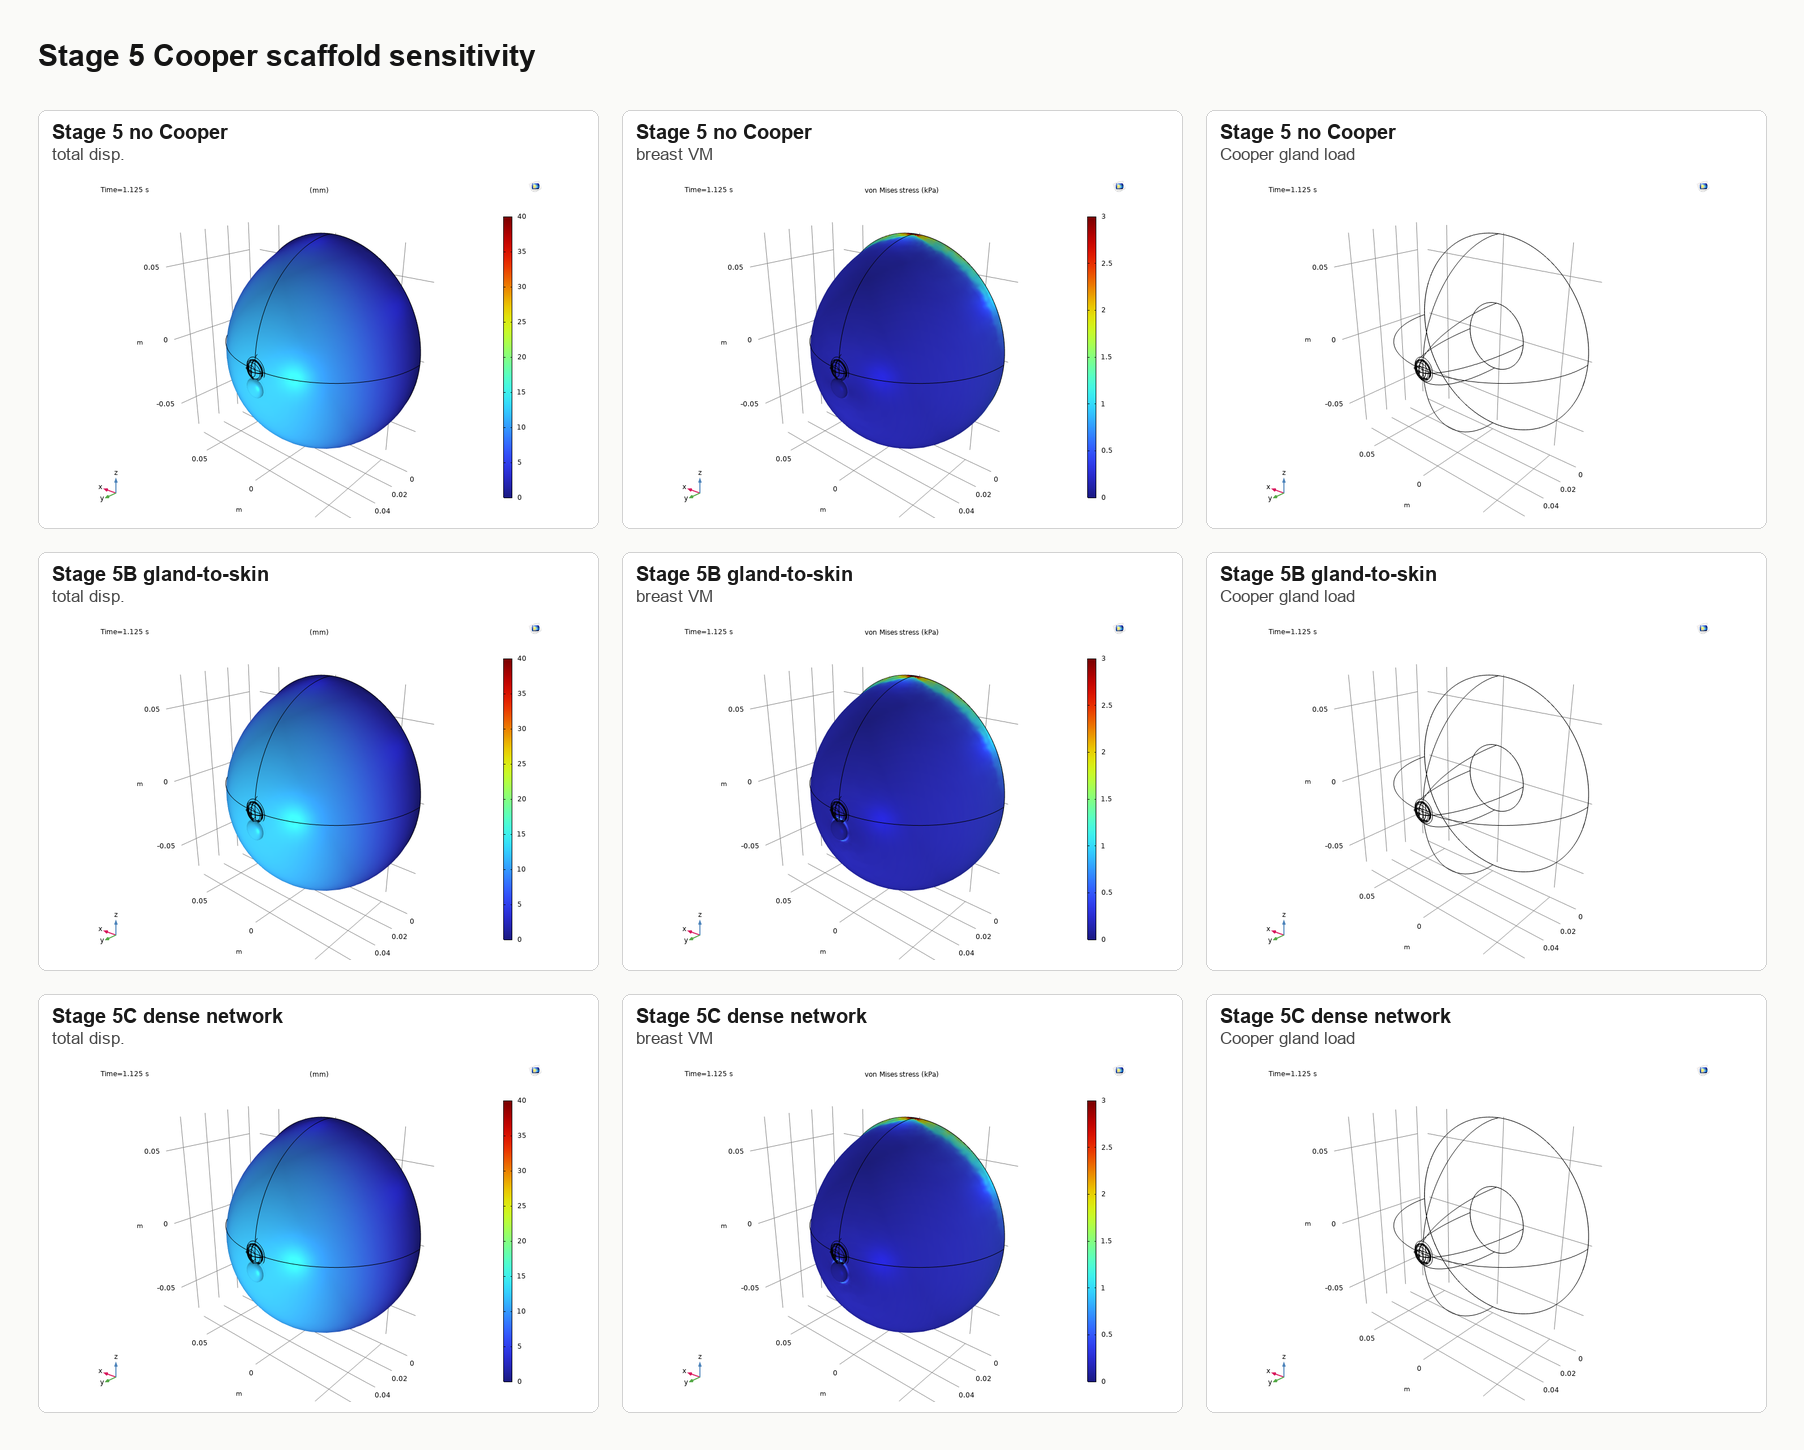
\includegraphics[width=0.95\linewidth,height=0.78\textheight,keepaspectratio]{Figures/comsol_contact_sheets/stage5_cooper_contact_sheet.png}
\caption{Source contact sheet for the Cooper-support development branch. The stable reference interpretation uses the no-Cooper control unless a Cooper-support variant solves robustly and produces complete post-processing output.}
\label{fig:appendix_stage5_figures}
\end{figure}

\addtocontents{toc}{\protect\setcounter{tocdepth}{2}}


\end{document}